\chapter{The fractional quaternion discrete Fourier transform and its applications}
\label{ch:FrQDFT}

Linear discrete transforms are building blocks for a multitude of techniques in the field of signal processing, being almost as important as they are diverse. Among the factors which distinguish one from the others, there is the algebraic structure over which they are defined, e.~g. a finite field and its extensions (such as in number-theoretic \parencite{blahut2010fast,pedrouzo2017number,chandra2014exact,lima2013} and arithmetic \parencite{knockaert1994generalized, rajapaksha2014vlsi} transforms), or the real and complex fields (as in the usual discrete Fourier transform). Let us recall an important point that has already been made: as the algebra is extended (for instance, from $ \mathbb{R} $ to $ \mathbb{C} $), it is possible to encode more information into each signal sample. Such was the motivation behind Sangwine's definition \parencite{sangwine1996fourier} of discrete two-dimensional quaternion transforms, based on their continuous counterparts previously defined by Ell \parencite{ell1993quaternion}: to apply these four-dimensional numbers --- the quaternions, an extension of the complex field --- to color image processing. Since then, quaternion transforms have been useful not only to image processing \parencite{ell2007hypercomplex,chen2018quaternion,li2013quaternion,evans2000hypercomplex,silva2018}, but also to other fields, such as bivariate signal analysis \parencite{flamant2017spectral,flamant2017time,flamant2018complete}.

Fractional transforms are yet another class of tools of great use, the reader may remember the review presented in Chapter \ref{ch:reviewGSP}. Regarding quaternion transforms, a couple of competent works have already addressed their fractionalization \parencite{guanlei2008fractional, wei2013different, roopkumar2016quaternionic} and some applications have been proposed \parencite{chen2018quaternion}. However, the author is not aware of papers approaching fractional quaternion discrete transforms \textit{from an eigenstructure analysis point of view}. This reasoning may unfold new theoretical insights and implementation techniques, and such is the motivation for this work.

In this chapter, the eigenstructure of the quaternion discrete Fourier transform (QDFT) matrix is investigated and shown to be closely related to that of the unitary discrete Fourier transform (DFT). This result offers an approach for defining the fractional version of the QDFT (referred to as FrQDFT). Following the central goal of defining the transform through eigendecomposition theory, a generalization is proposed in the form of a multiparametric fractional quaternion discrete Fourier transform (MFrQDFT). For illustrative purposes, this work proposes and briefly explores an encryption scheme for color images with opacity layer, fully harnessing the holistic processing of 4-channels 2D signals through the MFrQDFT.

The proposed method for image encryption fits in the class of schemes that use linear transforms alongside non-linear blocks \parencite{hsue2018enhancing}, to implement confusion and diffusion. The currently available methods in the state-of-the-art literature respond to a diverse range of needs, as fast implementation through parallel computing \parencite{wang2019fast}, increased safety and robustness by using matrix semi-tensor product \parencite{wang2020image} or one-time keys \parencite{liu2010}, just to name a few examples. The main scope of this chapter is not the encryption scheme \textit{per se}, but rather the FrQDFT eigenscructure and the MFrQDFT definition, the latter having the image encryption as a framework to showcase some of its possibilities. Nevertheless, the proposed encryption algorithm is described and evaluated to some extent. Although being an illustrative scenario, it stands on tools adopted currently by the literature. For example, the chosen method for key generation involved the use of chaotic maps, known to help achieving high bit sensibility and large key space. It follows works such as the one by Liu and Wang \parencite{liu2011color}, which proposed a color image encryption scheme using two chaotic maps and one-time keying, aiming to achieve large key space and cycle lengths. Another work by Liu and Wang \parencite{liu2012} employed a piecewise linear chaotic map and DNA encoding for ensuring the initial conditions of the encryption change according to the image, whereas Wang \textit{et al.} \parencite{wang2010chaotic} used a Lorentz chaotic map and a perceptron model applied to image encryption. The proposed scheme uses a chaotic tent map to generate a pseudo-random sequence, from which the secret parameters are extracted.


This chapter is structured as follows. Section \ref{sec:autoestrutura} presents the usual definition of the QDFT and proves the central theorem of this work, regarding how the DFT and QDFT share symmetric eigenvectors; it closes with comments on the quaternion representation of color images with opacity layer. Section \ref{sec:FrQDFT} discusses the fractionalization of the QDFT from an eigenstructure point of view and demonstrates some properties purely based on matrix algebra. Section \ref{sec:multi} proposes a multiparametric extension of the fractional transform and presents an application involving encryption of color images with opacity layer. The main results are summarized in Section \ref{sec:conclusao}.


\section{Eigenstructure of the QDFT}
\label{sec:autoestrutura}
Let us recall the definition of the 1D left QDFT of axis $ \qmu $ -- a unit pure quaternion, as presented in \parencite[Sec. 3.3.1]{ell2014quaternion} and in (\ref{eq:QDFT_fwd}). The $ m$-th entry of the QDFT of vector $ \mathbf{v} $ is
\begin{equation}
\label{eq:QDFT_fwd}
\!\widehat{v}_m \!=\! \text{QDFT}\{ \mathbf{v} \}_m \!\overset{\Delta}{=}\! \frac{1}{\sqrt{N}} \!\sum_{n=0}^{N-1}  \exp \left( -\qmu \frac{2\pi}{N} nm \right) v_n \!\in\! \mathbb{C}_{\qmu},\!
\end{equation}
in which $ \mathbb{C}_{\qmu} $ denotes the set of numbers $ a + \qmu b $, $ a,b \in \mathbb{R} $, isomorphic to the complex set. It matters to notice that, due to the lack of commutativity in quaternion multiplication, the position of the kernel relative to the operand in (\ref{eq:QDFT_fwd}) is relevant and must be kept consistent along all computations. Hence, the inverse transformation must be computed with the kernel on the same relative position,
\begin{equation}
\label{eq:QDFT_inv}
v_n = \text{QDFT}^{-1}\{ \widehat{\mathbf{v}} \}_n = \frac{1}{\sqrt{N}}\sum_{m=0}^{N-1}  \exp \left( \qmu \frac{2\pi}{N} nm \right) \widehat{v}_m.
\end{equation}

The synthesis and analysis equations may be written in matrix form as
\begin{equation}
\label{eq:QDFT}
\widehat{\mathbf{v}} = \text{QDFT}\{ \mathbf{v} \} = \mathbf{F} \mathbf{v},
\end{equation}
\begin{equation}
\label{eq:QDFT_mtx_inv}
\mathbf{v} = \text{QDFT}^{-1}\{ \widehat{\mathbf{v}} \} = \mathbf{F}^{-1} \widehat{\mathbf{v}},
\end{equation}
where $ \mathbf{F} $ is the unitary QDFT matrix, with entries $ \{\mathbf{F}\}_{n,m} = \sqrt{N}^{-1} \exp \left( -\qmu \frac{2\pi}{N} nm \right)$. Since $ \exp \left( -\qmu \frac{2\pi}{N} \right) $ is an $ N $-th root of unity, such as $ \exp \left( -\qi \frac{2\pi}{N} \right) $, it follows that $ \mathbf{F} $ shares many properties of the DFT matrix, such as invertibility (simple calculations show that $ \mathbf{F}^{-1} = \mathbf{F}^{H} $), what guarantees validity of the inversion formulae in (\ref{eq:QDFT_inv}) and (\ref{eq:QDFT_mtx_inv}).

The two-dimensional QDFT can be defined in a similar fashion, although more options regarding kernel positioning are available, since for any pure quaternions $ \qmu \neq \qnu $, one may verify that generally $ e^{\qnu \alpha} e^{\qmu \beta} \neq e^{\qnu \alpha + \qmu \beta} $. Ell and Sangwine \parencite{ell2014quaternion} presented the \textit{eight} distinct ways of building a 2D-QFT, which translate directly into options for 2D-QDFT. One of such possibilities is to transform the quaternion-valued matrix $ \mathbf{X} \in \mathbb{H}^{N\times M}$ according to the equation
\begin{equation}
\label{eq:2DQDFT-01}
\widehat{X}_{u,k} = 
\text{2D-QDFT}\{ \mathbf{X} \}_{u,k} \!\overset{\Delta}{=}\! \frac{1}{\sqrt{MN}} \!\sum_{n=0}^{N-1} \sum_{m=0}^{M-1}  \exp \left( -\qmu \frac{2\pi}{N} nu \right) X_{n,m} \exp \left( -\qnu \frac{2\pi}{M} mk \right).
\end{equation}
This formulation of the 2D-QDFT translates into the following matrix equation,
\begin{equation}
\label{eq:2DQDFT-02}
\widehat{\mathbf{X}} = \mathbf{F}^{(\qmu)} \mathbf{X} \mathbf{F}^{(\qnu)},
\end{equation}
where the Fourier matrices are similar to the one used in (\ref{eq:QDFT}), except from the pure quaternion which serves as transform axis (shown in the parenthesis). This is a consequence of the \textit{separability} of the 2D-QDFT, by which this transform may be conceived as the successive application of two 1D-QDFTs: once in the rows of $ \mathbf{X} $, once in the columns. Therefore, some results and properties derived for the 1D-QDFT may naturally extend to the two-dimensional case.

The similarities between the QDFT and the DFT matrices hugely aid the investigation of the eigenstructure of matrix $ \mathbf{F} $. As a result of Theorem \ref{th:01}, which is a contribution of this thesis, one is able to deduce the QDFT eigenstructure out of even and odd DFT eigenvectors, by using a variation of Pei's reasoning regarding the 2D-QDFT \parencite{pei2010eigenfunctions}.

\begin{theorem}
\label{th:01}
Let $ \mathbf{v} $ be an eigenvector of the unitary DFT with eigenvalue $ \lambda $.
\begin{itemize}[noitemsep]
\item[(a)] If $ \mathbf{v} $ has even symmetry (in which case $ \lambda = \pm 1 $), then it is also an eigenvector of the QDFT with eigenvalue $ \lambda $.
\item[(b)] If $ \mathbf{v} $ has odd symmetry (in which case $ \lambda = \pm \qi $), then it is also an eigenvector of the QDFT (of axis, let us say, $ \qmu $) with eigenvalue $ -\lambda \qi \qmu$, i.~e., $ \pm \qmu $.
\end{itemize}
\end{theorem}

\begin{proof}
\begin{itemize}
\item[(a)] If $ \mathbf{v} $ has even symmetry, i.~e., $ v_n = v_{N-n} $ for $ n=1,\dots,N-1 $, then
\begin{equation}
%\label{key}
\sum_{n=0}^{N-1} v_n \sin \frac{2\pi}{N} nm = 0,
\end{equation}
therefore,
\newcommand{\correctinghspace}{-1.8cm}
% \begin{equation*}
%\small
% \label{eq:15}
\begin{align*}
\sqrt{N} \text{QDFT}\{ \mathbf{v} \}_m &= \sum_{n=0}^{N-1} v_n e^{-\qmu \frac{2\pi}{n} nm} \\
&\hspace{\correctinghspace}
=\sum_{n=0}^{N-1} v_n \left( \cos \frac{2\pi}{n} nm - \qmu \sin \frac{2\pi}{n} nm \right) \\
&\hspace{\correctinghspace}
= \left( \sum_{n=0}^{N-1} v_n \cos \frac{2\pi}{n} nm \right) - \underbrace{\left(  \sum_{n=0}^{N-1} v_n \sin \frac{2\pi}{n} nm \right)}_{=0} \qmu \\
&\hspace{\correctinghspace}
= \left( \sum_{n=0}^{N-1} v_n \cos \frac{2\pi}{n} nm \right) - \underbrace{\left(  \sum_{n=0}^{N-1} v_n \sin \frac{2\pi}{n} nm \right)}_{=0} \qi \\
&\hspace{\correctinghspace}
= \sqrt{N} \text{DFT}\{ \mathbf{v} \}_m = \sqrt{N} \lambda v_m \\
&\hspace{\correctinghspace}
\Rightarrow \text{QDFT}\{ \mathbf{v} \} = \lambda \mathbf{v}.
\end{align*}
% \end{equation*}
\item[(b)] If $ \mathbf{v} $ has odd symmetry, i.~e., $ v_n = -v_{N-n} $ for $ n=1,\dots,N-1 $ and $ v_0 = 0 $, then
\begin{equation}
%\label{key}
\sum_{n=0}^{N-1} v_n \cos \frac{2\pi}{N} nm = 0,
\end{equation}
hence,
\begin{equation}
\small
\label{eq:17}
\begin{aligned}
\sqrt{N} \text{QDFT}\{ \mathbf{v} \}_m &= \sum_{n=0}^{N-1} v_n e^{-\qmu \frac{2\pi}{n} nm}\\
&\hspace{\correctinghspace}
=
\sum_{n=0}^{N-1} v_n \left( \cos \frac{2\pi}{n} nm - \qmu \sin \frac{2\pi}{n} nm \right) \\
&\hspace{\correctinghspace}
= {\underbrace{\left( \sum_{n=0}^{N-1} v_n \cos \frac{2\pi}{n} nm \right)}_{=0} - \left(  \sum_{n=0}^{N-1} v_n \sin \frac{2\pi}{n} nm \right) \qmu }\\
&\hspace{\correctinghspace}
= - \left(  \sum_{n=0}^{N-1} v_n \sin \frac{2\pi}{n} nm \right) \qmu.
\end{aligned}
\end{equation}

But, from the odd symmetry assumption,
\begin{equation}
%\label{key}
\begin{aligned}
\sqrt{N}\lambda v_m = \sqrt{N}\text{DFT}\{ \mathbf{v} \}_m &= \sum_{n=0}^{N-1} v_n e^{-\qi \frac{2\pi}{n} nm}= - \left(  \sum_{n=0}^{N-1} v_n \sin \frac{2\pi}{n} nm \right) \qi,
\end{aligned}
\end{equation}
therefore (remember that $ \lambda $ and $ v_m $ commute)
\begin{equation}
\label{eq:19}
\sum_{n=0}^{N-1} v_n \sin \frac{2\pi}{n} nm = \sqrt{N}v_m \lambda \qi.
\end{equation}
From (\ref{eq:17}) and (\ref{eq:19}),
\begin{equation}
\label{eq:20}
\begin{aligned}
\sqrt{N}\text{QDFT}\{ \mathbf{v} \}_m &=  -\sqrt{N}\text{DFT} \{ \mathbf{v} \}_m \qi \qmu \\
&\hspace{\correctinghspace}
= -\sqrt{N}v_m \lambda \qi \qmu \\
&\hspace{\correctinghspace}
\Rightarrow \text{QDFT}\{ \mathbf{v} \} = -\lambda \qi \qmu \mathbf{v}.
\end{aligned}
\end{equation}
\end{itemize}
\end{proof}

The results of Theorem \ref{th:01} are summarized in Table \ref{tab:01}.
This analysis can immediately be extended to the two-dimensional case if one considers the separability of the 2D-QDFT, mentioned after (\ref{eq:2DQDFT-02}). If $ (\mathbf{e}^{(\qmu)}, \lambda_{\qmu}) $ and $ (\mathbf{e}^{(\qnu)}, \lambda_{\qnu}) $ are (column-)eigenvector-eigenvalue pairs of the matrices $ \mathbf{F}^{(\qmu)} $ and $ \mathbf{F}^{(\qnu)} $, respectively, then the 2D signal $ \mathbf{e}^{(\qmu)} \mathbf{e}^{(\qnu)^T}  $ is a 2D-QDFT eigenvector with eigenvalue $ \lambda_{\qmu} \lambda_{\qnu} $ \parencite{candan2011}. Therefore, this 2D-QDFT has eight (possibly) distinct eigenvalues: $ \pm 1, \pm \qmu, \pm \qnu, \pm \qmu \qnu $.

\begin{table}[b!]
\center
\captionof{table}{DFT and QDFT eigenvectors.}
\label{tab:01}
\begin{tabular}{ccc}
\toprule
\shortstack{Eigenvector\\ symmetry} & \shortstack{Eigenvalue\\(DFT)} & \shortstack{Eigenvalue\\(QDFT)} \\
\midrule
Even & $ \pm 1 $ & $ \pm 1 $ \\
Odd & $ \pm \qi $ & $ - (\pm \qi) \qi \qmu = \pm \qmu $\\
\bottomrule
\end{tabular}
\end{table}

\subsection{2D-QDFT and color images with opacity layer}
\label{subsec:2D_QDFT}
The 2D-QDFT has been commonly used to process color images, which are represented as matrices of pure quaternions \parencite{lu20072d,ell2006hypercomplex,chen2018multiple}. In this representation, each color channel of a certain pixel corresponds to an imaginary component of the pure quaternion. Although this mapping is useful and adequate, it neglects the quaternion scalar part (always set to zero), causing a difference in dimensionality between input and output of the 2D-QDFT: while the image is a 2D signal with three-dimensional components, its spectrum has four-dimensional entries. It surely is not a problem \textit{per se}, rather is an inconvenience, also found when processing real signals with the DFT.

An application free from this inconvenience is the analysis of color images with opacity (or alpha) layer, as in files in portable network graphics format (PNG). In this case, each pixel $ (R,G,B,\alpha) $ is mapped into $ q = \alpha + R \qi + G \qj + B \qk $, forming the quaternion-valued matrix $ \mathbf{X} $. Let us compute the 2D-QDFT by separately transforming the rows and columns using (\ref{eq:2DQDFT-02}), with the same transform axis on both sides,
\begin{equation}
\label{eq:2DQDFT}
\text{2D-QDFT}\{\mathbf{X} \} = \mathbf{F} \mathbf{X} \mathbf{F}^T.
\end{equation}

One should notice that the transformation in (\ref{eq:2DQDFT}) does \textit{not} consist on the successive application of the \textit{same} QDFT to the rows and columns of matrix $ \mathbf{X} $. Due to the noncommutative nature of quaternion multiplication, as it was previously mentioned, different transforms are obtained when choosing between left- or right-multiplications, even though the transform axis is kept unchanged. The operation in (\ref{eq:2DQDFT}) performs a \textit{left} QDFT on the columns and a \textit{right} QDFT on the rows, as it is clear from (\ref{eq:2DQDFT-01}). A 2D-QDFT consisting of the \textit{same} transformation applied in both dimensions must use multiplications with the same orientation, e.~g.
\begin{equation}
\label{eq:2DQDFTv2}
\mathbf{F} \left( \mathbf{F}\mathbf{X}^T \right)^T.
\end{equation}

Fig. \ref{fig:2D_QDFTv1} shows the QDFT -- according to (\ref{eq:2DQDFT}) -- of Fig. \ref{fig:dice}, as another PNG image. As an illustration of the difference in using (\ref{eq:2DQDFT}) or (\ref{eq:2DQDFTv2}), caused by the lack of commutativity in quaternion multiplication, the mean squared error (MSE) between the two spectra was computed. The result was approximately 1070. % Cálculo feito com o script trying_separable_2DQDFT.py


%{\color{red}(Mantemos isso?) \'E curioso observar que, ao processar imagens em PNG utilizando a 2D-QDFT, tanto o sinal (imagem) de entrada como o de sa\'ida s\~ao compostos por quaternions (geralmente) n\~ao-puros, o que permite usar a mesma representa\c c\~ao no dom\'inio do sinal e da transformada. Ao usar a 2D-DFT para processar imagens em escala de cinza, ou a 2D-QDFT para imagens em RGB, o dom\'inio espectral difere daquele do sinal original.}

\begin{figure}
\centering
\subfloat[\label{fig:2D_QDFTv1}]{
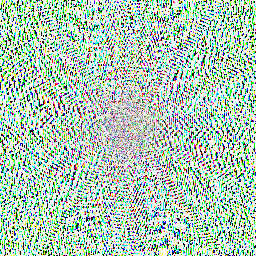
\includegraphics[width=0.3\linewidth]{Figures/2D_QDFTv1.png}
}~
\subfloat[\label{fig:2D_QDFTv2}]{
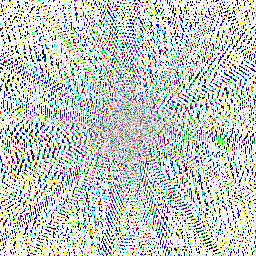
\includegraphics[width=0.3\linewidth]{Figures/2D_QDFTv2.png}
}
\caption{(a) 2D-QDFT of the PNG image in Fig. \ref{fig:dice}, according to (\ref{eq:2DQDFT}), with axis $ \qmu = \frac{1}{\sqrt{3}}(\qi + \qj + \qk) $. (b) 2D-QDFT of the same image, same transform axis, following the approach in (\ref{eq:2DQDFTv2}).}
\label{fig:QDFT}
\end{figure}

\section{The fractional quaternion discrete Fourier transform}
\label{sec:FrQDFT}
The proposed fractionalization method for the QDFT explores the eigenvector sharing between the DFT and the QDFT: as long as one possesses an orthogonal eigenvector matrix $ \mathbf{E} $ for the DFT, it can be used for the QDFT matrix diagonalization and its subsequent fractionalization. For instance, the eigendecomposition of the DFT matrix allows to find its fractional counterpart by raising each eigenvalue to a non-integer parameter $ a $, i.~e.

\begin{equation}
\label{eq:FrDFT}
\mathbf{F}_{\text{DFT}}^a = \mathbf{E} \mathbf{\Lambda}^a \mathbf{E}^T,
\end{equation}
where $ \mathbf{\Lambda} $ is the diagonal matrix containing the DFT eigenvalues.

Oliveira Neto and Lima \parencite{de2017discrete} stress that a FrDFT expressed as in (\ref{eq:FrDFT}) will numerically approximate its continuous version if and only if the columns of $ \mathbf{E} $ approximate samples of continuous Hermite-Gaussian functions. In \parencite{de2017discrete}, the authors present two methods to generate such an orthogonal eigenbasis, one of which (the generating matrix method) is the one adopted in this work.

\begin{figure*}
\centering
\subfloat[\label{fig:dice}]{
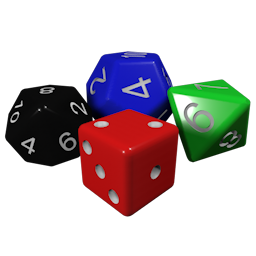
\includegraphics[width=0.25\linewidth]{Figures/dice_256x256.png}
}~
\subfloat[]{
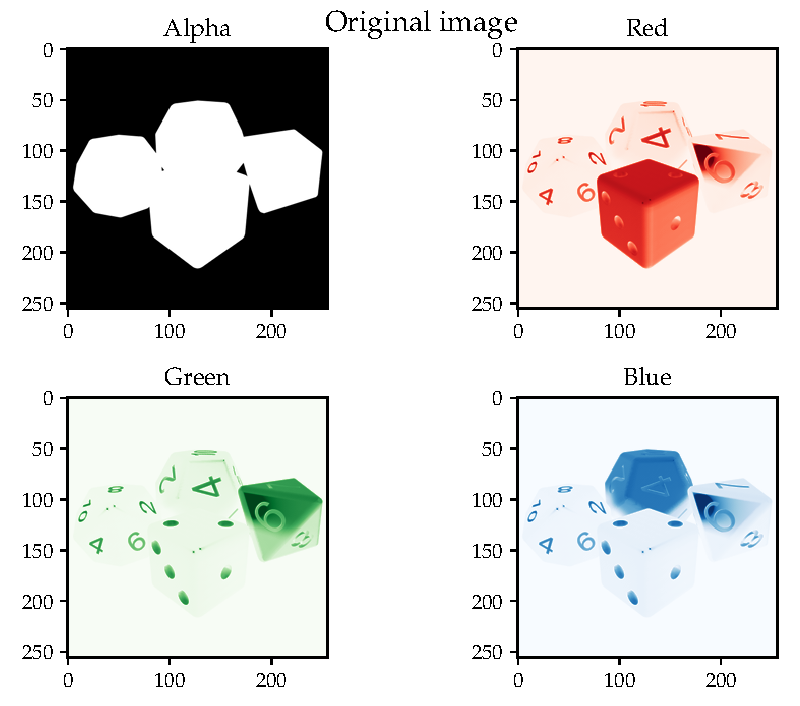
\includegraphics[width=0.355\linewidth]{Figures/dice_256x256_layers.pdf}
}~
\subfloat[]{
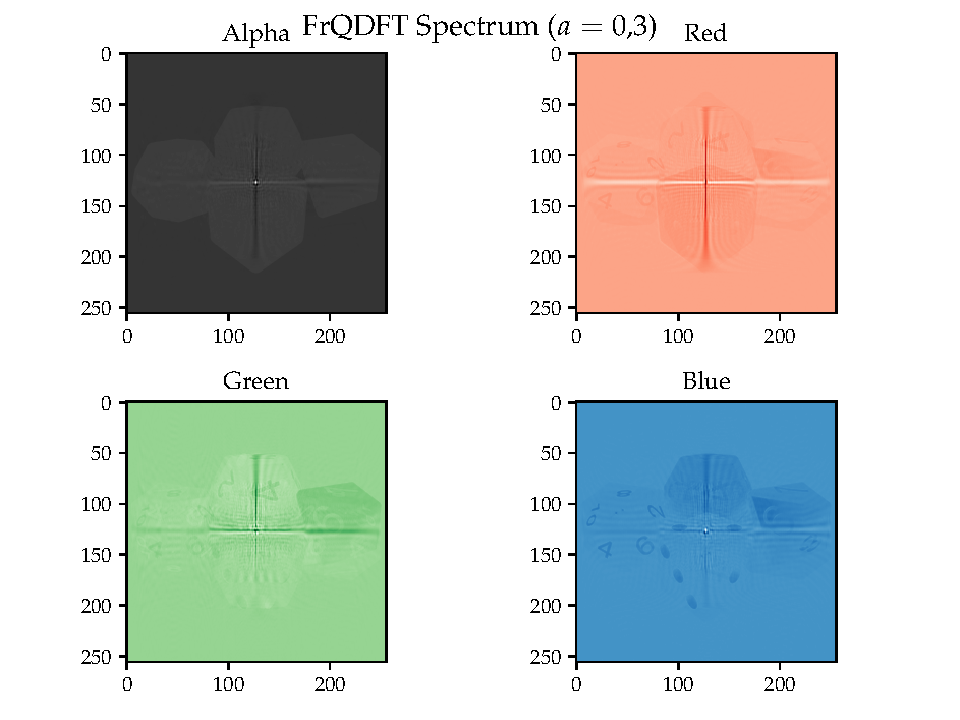
\includegraphics[width=0.355\linewidth]{Figures/dice_256x256_layers_frqdft.pdf}
}~
\caption{(a) Test PNG image. Visualization of each layer in the (b) test image and (c) in its FrQDFT spectrum, computed with transform axis $ \qmu = \frac{1}{\sqrt{3}}(\qi + \qj + \qk) $ and $ a=0{.}3 $.}
\end{figure*}

Once one is able to compute an orthogonal eigenbasis $ \mathbf{E} $ containing Hermite-Gaussian-like DFT eigenvectors, for instance by means of the generating matrix method, Theorem \ref{th:01} assures that matrix $ \mathbf{E} $ is also an eigenvector matrix for the QDFT. As a consequence, the transform matrix $ \mathbf{F} $ may be decomposed and written as
\begin{equation}
\label{eq:QDFTmtx}
\mathbf{F} = \mathbf{E} \mathbf{\Gamma} \mathbf{E}^T,
\end{equation}
in which the diagonal matrix $ \mathbf{\Gamma} $ is obtained by replacing $ \qi $ with $ \qmu $ in $ \mathbf{\Lambda} $ (Table \ref{tab:01}). Therefore, the \textit{fractional} quaternion Fourier transform, or simply FrQDFT, is obtained by raising each eigenvalue in $ \mathbf{\Gamma} $ to a so-called fractional order $ a \in \mathbb{R} $, so that
\begin{equation}
\label{eq:QDFTmtxa2}
\text{FrQDFT}_a\{ \mathbf{v} \} \overset{\Delta}{=} \mathbf{F}^a \mathbf{v},
\end{equation}
%\ref{eq:QDFTmtx}
where
\begin{equation}
\label{eq:QDFTmtxa}
\mathbf{F}^a = \mathbf{E} \mathbf{\Gamma}^a \mathbf{E}^T.
\end{equation}

The FrQDFT, as defined in (\ref{eq:QDFTmtxa2}) and (\ref{eq:QDFTmtxa}), possesses all the classical properties of a fractional Fourier transform:

\begin{itemize}
\item \textit{Reduction to the ordinary quaternion transform}: if $ a=1 $, then the synthesis equation in (\ref{eq:QDFTmtxa2}) equals (\ref{eq:QDFT}), coinciding with the QDFT. The proof is imediate.

\item \textit{Reduction to the identity}: if $ a=0 $, the FrQDFT reduces to the identity operator, represented as $ \mathbb{I} $.

\begin{proof}
From the orthogonality of the eigenvector matrix $ \mathbf{E} $,
\begin{equation}
%\label{key}
\mathbf{F}^0 = \mathbf{E} \mathbf{\Gamma}^0 \mathbf{E}^T = \mathbf{E} \mathbf{E}^T = \mathbb{I}.
\end{equation}
\end{proof}

\item \textit{Index addititivy}: applying the FrQDFT twice, using $ a $ and $ b $ as fractional orders, equals applying a single FrQDFT with fractional order $ a+b $. Equivalently, $ \mathbf{F}^a \mathbf{F}^b = \mathbf{F}^{a+b} $.

\begin{proof}
\begin{equation}
%\label{key}
\begin{aligned}
\mathbf{F}^a \mathbf{F}^b &= \mathbf{E} \mathbf{\Gamma}^a \mathbf{E}^T
\mathbf{E} \mathbf{\Gamma}^b \mathbf{E}^T \\
&= \mathbf{E} \mathbf{\Gamma}^a \mathbf{\Gamma}^b \mathbf{E}^T,
\end{aligned}
\end{equation}
but, since $ \mathbf{\Gamma} $ is a diagonal matrix, $ \mathbf{\Gamma}^a \mathbf{\Gamma}^b =
\mathbf{\Gamma}^{a+b} $, hence
\begin{equation}
%\label{key}
\mathbf{F}^a \mathbf{F}^b = \mathbf{E} \mathbf{\Gamma}^a \mathbf{\Gamma}^b \mathbf{E}^T = \mathbf{E} \mathbf{\Gamma}^{a+b} \mathbf{E}^T =
\mathbf{F}^{a+b}.
\end{equation}
\end{proof}

\item \textit{Unitary matrix}: the matrix $ \mathbf{F}^a $ is unitary, i.~e.
\begin{equation}
%\label{key}
\mathbf{F}^a (\mathbf{F}^a)^H = \mathbb{I},
\end{equation}
in which $ (\cdot)^H $ denotes the Hermitian (conjugate transpose) operator.
%\footnote{The \textit{quaternion} conjugation is considered, i.~e., se $ q = a + b\qi + c\qj + d\qk = r \exp (\qmu \theta) $, ent\~ao seu conjugado \'e $ \bar{q} = a - b\qi - c\qj - d\qk = r \exp (-\qmu \theta) $}

\begin{proof}
Since all FrQDFT eigenvalues $ \gamma_n $ are fourth roots of unity in the 1-$\qmu $ plane (i.~e., $ \gamma_n = \pm 1, \pm \qmu $ and, therefore, it has unit module), they can be written as $ \gamma_n = \exp \qmu \theta $ (in which $ \theta = 0, \pm \frac{\pi}{2}, \pi $). Hence
% ent\~ao podem ser escritos na forma $ \gamma_n = \exp \qmu \theta $ (em que $ \theta = 0, \pm \frac{\pi}{2}, \pi $). Assim,
\begin{equation}
%\label{key}
\overline{\gamma^a_n} = \gamma_n = \exp (-a \qmu \theta) = \gamma^{-a}_n,
\end{equation}
consequently
\begin{equation}
\label{eq:24}
(\mathbf{\Gamma}^a)^H = \mathbf{\Gamma}^{-a}.
\end{equation}

From (\ref{eq:24}) and (\ref{eq:QDFTmtxa}),
\begin{equation}
%\label{key}
\begin{aligned}
%\label{key}
(\mathbf{F}^a)^H &=  \left((\mathbf{E} \mathbf{\Gamma}^a) \mathbf{E}^T \right)^H =  \mathbf{E} \left(\mathbf{E} \mathbf{\Gamma}^a  \right)^H =
\mathbf{E} (\mathbf{\Gamma}^{a})^H \mathbf{E}^T = \mathbf{E} \mathbf{\Gamma}^{-a} \mathbf{E}^T = \mathbf{F}^{-a},
\end{aligned}
\end{equation}
and, following the index additivity and the reduction to identity properties,
\begin{equation}
%\label{key}
\begin{aligned}
%\label{key}
\mathbf{F}^a (\mathbf{F}^a)^H = \mathbf{F}^a \mathbf{F}^{-a} = \mathbf{F}^0= \mathbb{I}.
\end{aligned}
\end{equation}
\end{proof}
\end{itemize}

Before proceeding, it matters to notice that other approaches have been used to define fractional transforms especially suited for image encryption. Lima \textit{et al.} \parencite{figueiredo2018} applied the generating matrix method to obtain eigenvectors --- in a fashion similar to this work --- and define multiorder reality-preserving discrete fractional transforms. Roopkumar \parencite{roopkumar2016quaternionic}, on the other hand, defined a {continuous} one-dimensional quaternion fractional Fourier transform by using a reasoning similar to the symplectic decomposition of quaternions: adding together two traditional fractional Fourier operators with certain imaginary unit, with one of them multiplied by an orthogonal pure quaternion. None of the approaches, to the best of the author's knowledge, made use of eigenstructure analysis to define the FrQDFT and prove some of its properties.

\section{The multiparametric FrQDFT with application to color image encryption}
\label{sec:multi}
Frequently, fractional transforms are employed in both grayscale \parencite{tao2010image} and color image \parencite{kang2018reality, kang2018color} encryption. By setting the secret key to be the transform fractional order, alongside the use of multiple encryption or multiparametric transforms, one is able to create ciphers with sufficiently large key spaces and highly sensible to small key changes. This section presents an illustrative application of the FrQDFT, creating a holistic encryption scheme for PNG images based on the proposition of a multiparametric FrQDFT.

The definition of the multiparametric FrQDFT, referred to as MFrQDFT, consists of employing a different fractional order for each eigenvalue in $ \mathbf{\Gamma} $. The vector of fractional orders is represented by $ \mathbf{a} = [a_0, a_1, \dots, a_{N-1}] $. The MFrQDFT of a column vector $ \mathbf{v} $ is
\begin{equation}
\label{eq:MFrQDFT}
\text{MFrQDFT}\{ \mathbf{v} \} = \mathbf{E} \mathbf{\Gamma^a} \mathbf{E}^T \mathbf{v} = \mathbf{F^a} \mathbf{v}.
\end{equation}

The symbols $ \mathbf{\Gamma^a} $ and $ \mathbf{F^a} $ in (\ref{eq:MFrQDFT}) are abuses of notation. One must comprehend $ \mathbf{\Gamma^a} $ as the diagonal matrix obtained after raising the $ n $-th entry in the diagonal of $ \mathbf{\Gamma} $ to the $ n $-th component in $ \mathbf{a} $. On the other hand, $ \mathbf{F^a} $ indicates the matrix $ \mathbf{E} \mathbf{\Gamma^a} \mathbf{E}^T $. As it was done in Subsection \ref{subsec:2D_QDFT}, the 2D-MFrQDFT of a quaternion matrix $ \mathbf{X} $, e.~g. representing a PNG matrix, is written as
\begin{equation}
\label{eq:2DMFrQDFT}
\text{2D-MFrQDFT}\{\mathbf{X} \} \overset{\Delta}{=} \mathbf{\widehat{X}} = \mathbf{F^a} \mathbf{X} \mathbf{F^a}^T,
\end{equation}
with inverse transform obtained from the properties listed in Section \ref{sec:FrQDFT}
\begin{equation}
\label{eq:2DMFrQDFTinv}
\text{2D-MFrQDFT}^{-1}\{ \mathbf{\widehat{X}} \} = (\mathbf{F^a}^H) \mathbf{\widehat{X}} (\overline{\mathbf{F^a}}).
\end{equation}

\begin{figure*}
\centering
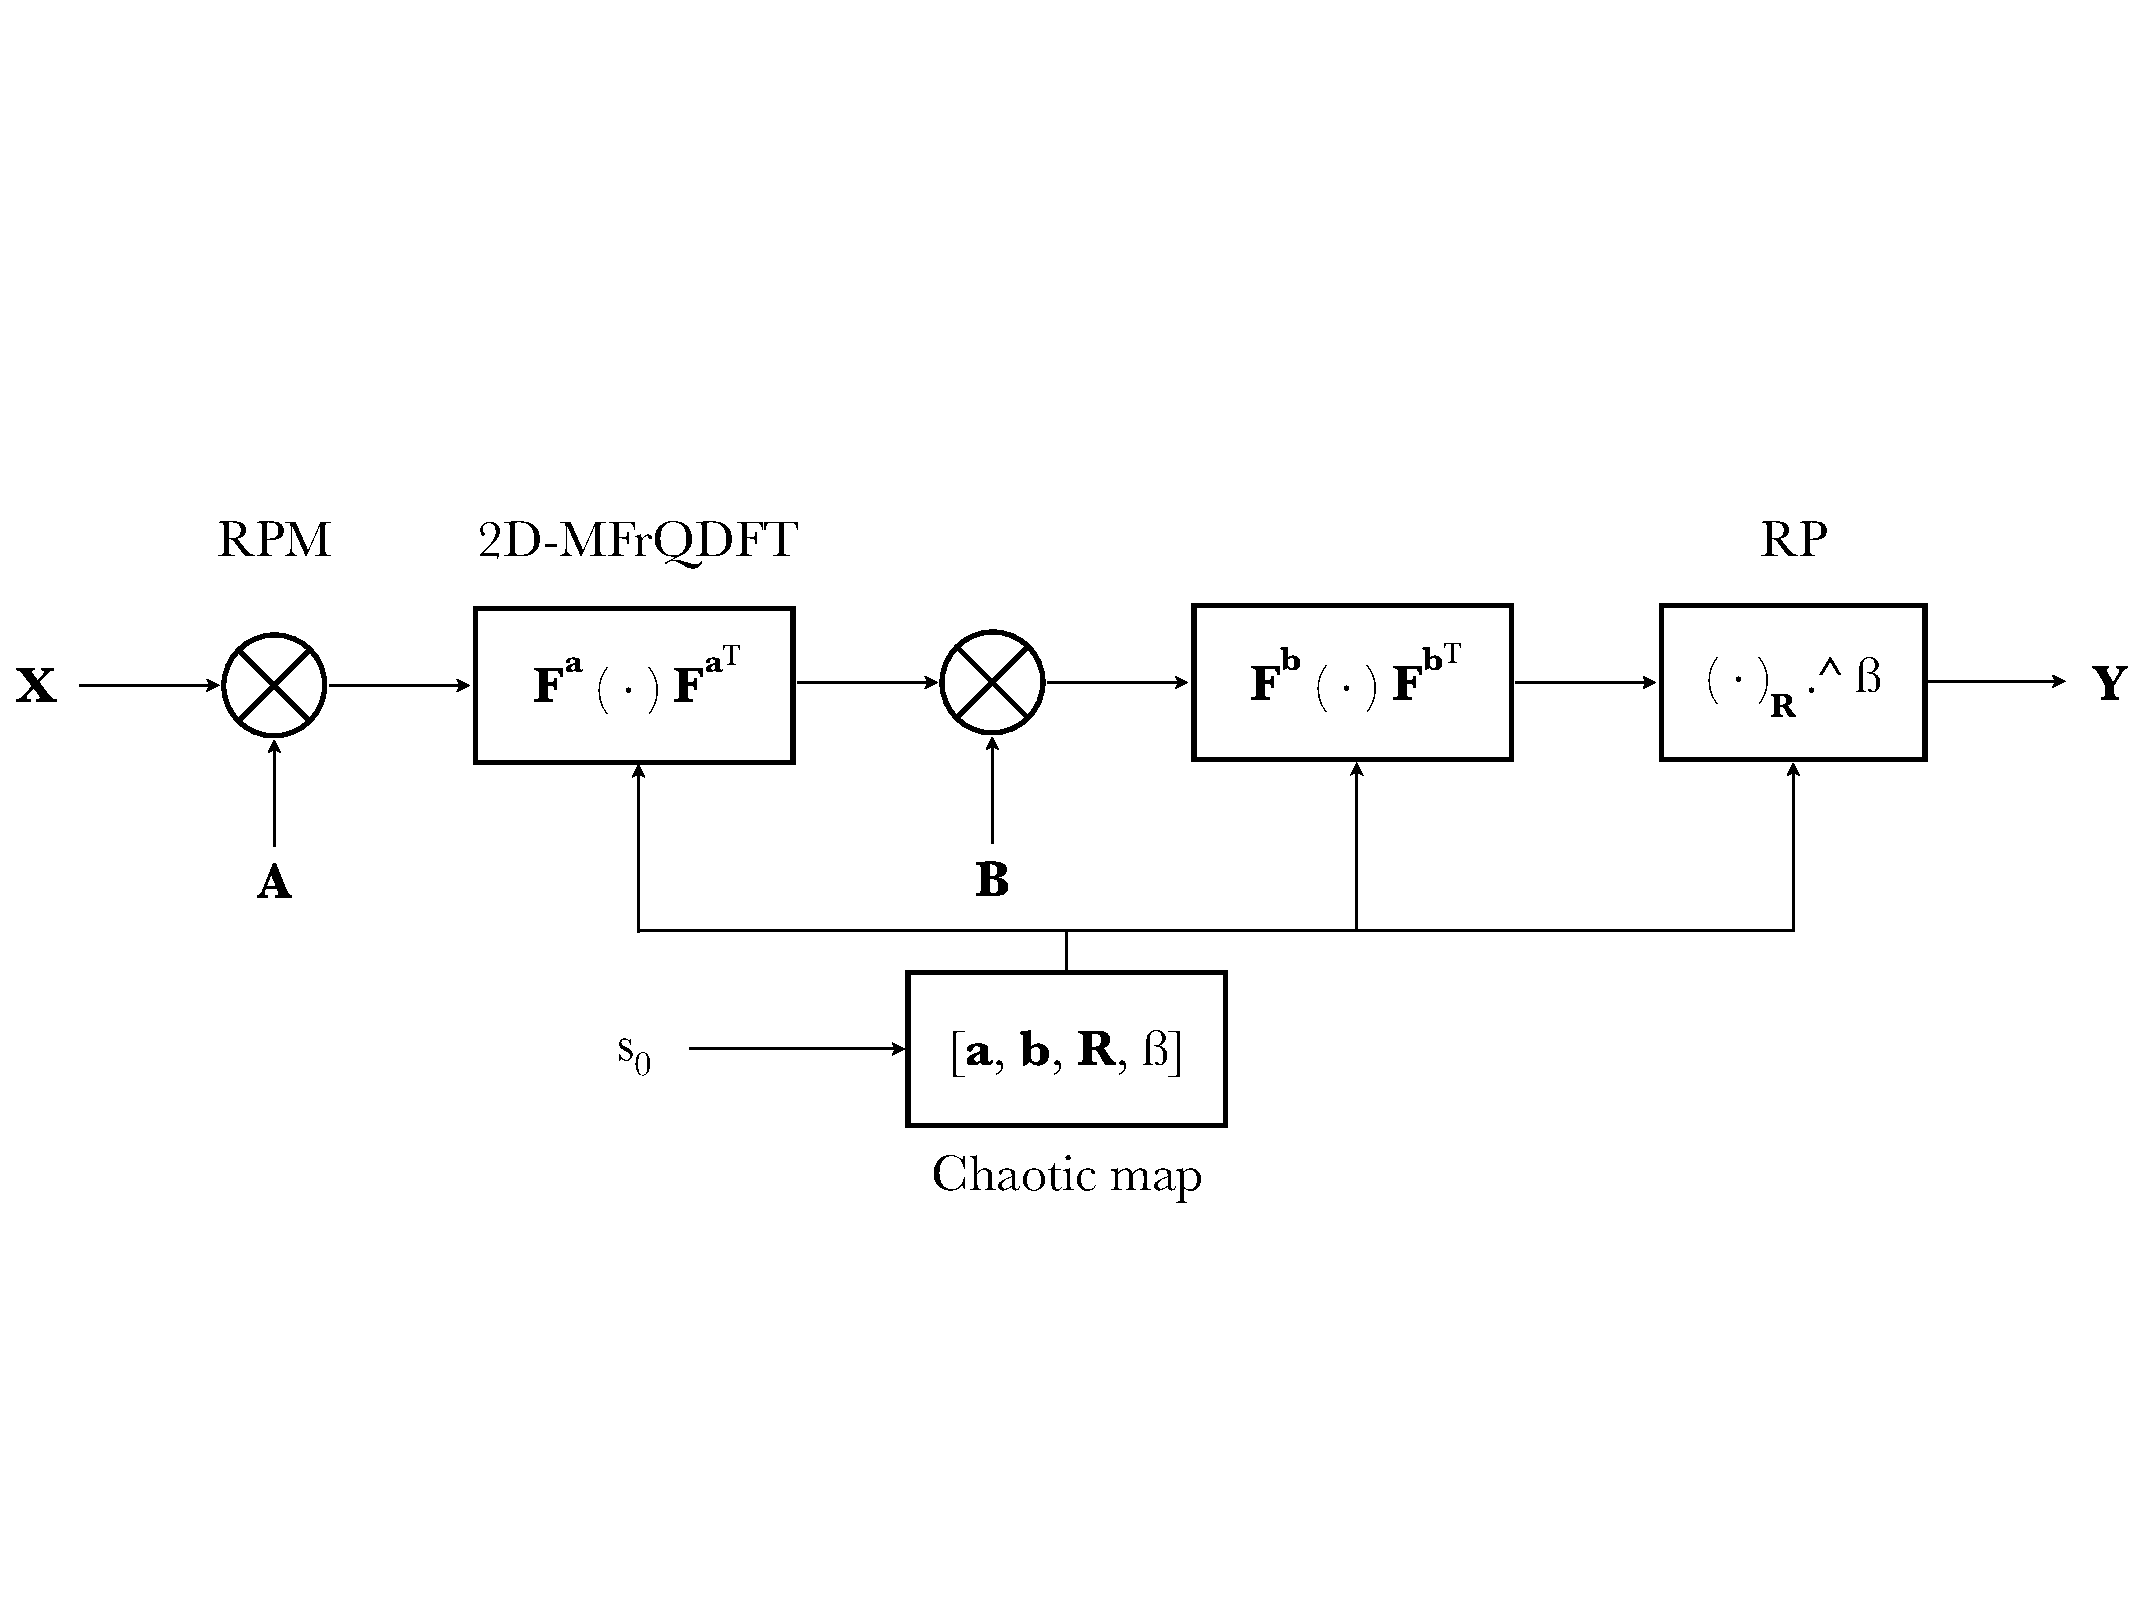
\includegraphics[width=0.9\linewidth]{Figures/esquema_EN.pdf}
\caption{Proposed encryption scheme, exploring the 2D-MFrQDFT.}
\label{fig:cifragem}
\end{figure*}

\begin{figure*}
\centering
\subfloat[\label{fig:ciphered01}]{
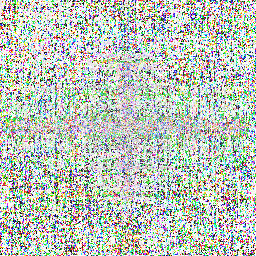
\includegraphics[width=0.2\linewidth]{Figures/sage_Encrypted_image.png}
}~
\subfloat[\label{fig:ciphered02}]{
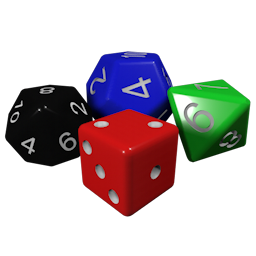
\includegraphics[width=0.25\linewidth]{Figures/Decrypted_image_error_0.png}
}~
\subfloat[\label{fig:ciphered03}]{

\includegraphics[width=0.2\linewidth]{Figures/sage_Decrypted_image_error_minus1dot6.png}
}~
\caption{(a) Encrypted image. (b) Image decrypted with the correct key $ s_0 $. (c) Image decrypted with the wrong key $ \widetilde{s_0} = s_0 + \epsilon $, with $ \epsilon = -1{,}6 \cdot 10^{-80} $.}
\end{figure*}

\subsection{Encryption scheme using MFrQDFT}

The chosen implementation for the PNG image encryption algorithm mixed a block of random-phase modulation (RPM, also called phase mask in \parencite{chen2018multiple} and \parencite{singh2008optical}) and multiparametric transform. As suggested by \parencite{hsue2018enhancing}, a non-linear step of random power is also used. Fig. \ref{fig:cifragem} depicts the system building blocks.

The plaintext image is initially converted into a quaternion matrix $ \mathbf{X} $, which is input to a 2-round processing with RPM $ + $ 2D-MFrQDFT. The random-phase modulation consists of element-wise multiplication by a matrix of random unit quaternions. This role is fulfilled by matrices $ \mathbf{A} $ and $ \mathbf{B} $ in Fig. \ref{fig:cifragem}. The \textit{inverse} RPM (in decryption) is achieved using the \textit{conjugate} of the matrix used during encryption.

The random-power block (RP) is the final step in the encryption method. It creates non-linearity by raising randomly selected entries of the matrix $ \mathbf{X} $ to a random parameter $ \beta \in \ ]0,1[$. This selection is performed by a binary matrix $ \mathbf{R} $, so that the output of the RP block to an input quaternions matrix $ \mathbf{M} $ is
\begin{equation}
%\label{key}
\text{RP}(\mathbf{M})_{i,j} =
\begin{cases}
(\mathbf{M}_{i,j})^\beta & \text{if } \mathbf{R}_{i,j} = 1, \\
\mathbf{M}_{i,j} & \text{if } \mathbf{R}_{i,j} = 0.
\end{cases}
\end{equation}
During decryption, one must use the same matrix $ \mathbf{R} $ and an exponent $ \beta^{-1} $.

A chaotic map was used to generate a pseudorandom sequence $ \mathbf{s} $ of numbers between 0 and 1, from which all of the encryption parameters were drawn: the fractional order vectors $ \mathbf{a} $ and $ \mathbf{b} $ of the two 2D-MFrQDFTs, the parameter $ \beta $ and the matrix $ \mathbf{R} $\footnote{For each entry $ \mathbf{R}_{i,j} $, a corresponding element $ s_k $ of $ \mathbf{s} $ was taken and $ \mathbf{R}_{i,j} $ was set to 1 if and only if $ s_k > 0{,}5 $, $ \mathbf{R}_{i,j} = 0 $ otherwise.} for the RP block. The random-phase modulation matrices were produced beforehand and could be left public in the scheme documentation. The encryption of a $ 256 \times 256 $-pixels image, therefore, requires a sequence of length $ 256 + 256 + 256^2 + 1  $. The secret key consists of the seed $ s_0 $ of the chaotic map, a floating point variable between 0 and 1.
%It is clear how the key space and the scheme security depend on the seed floating-point precision and the chosen chaotic map randomness.
As a consequence, the key space is determined by the smallest deviation $ \epsilon $ from $ s_0 $ so that, using the wrong key $ \widetilde{s_0} = s_0 \pm \epsilon $ in decryption, it still leads to a noisy image without any detectable trace of original information.

The key space dimension, denoted by $ [K] $, is the ratio between the range of all possible keys and the range of wrong keys \textit{which still lead to partial image reconstruction}. The latter is $ [s_0 - \epsilon, s_0 + \epsilon] $, following the previous definition of $ \epsilon $. Since $ s_0 \in \ ]0,1[ $,
\begin{equation}
%\label{key}
[K] = \frac{1 - 0}{s_0 + \epsilon - (s_0 - \epsilon)} = \frac{1}{2 \epsilon}.
\end{equation}

When testing the encryption scheme, the \textit{tent map} \parencite{singh2008optical} was chosen as tool for generating the $ \mathbf{s} $ sequence; it is recursively defined as
\begin{equation}
%\label{key}
s_{n+1} =
\begin{cases}
\gamma s_n & \text{if } 0 \leq s_0 < 0{.}5, \\
\gamma(1 - s_n) & \text{if } 0{.}5 \leq s_0 \leq 1.
\end{cases}
\end{equation}
with $0 <  \gamma \leq 2 $.

The tent map parameters were set to $ s_0 = 0{.}3 $ and $ \gamma = 1{.}8 $, for no particular reason other than obeying the range of values for chaotic behaviour. The proposed encryption algorithm was used on the image in Fig. \ref{fig:dice}, what yielded the ciphered output in Fig. \ref{fig:ciphered01}.

In order to evaluate the key space dimension, the ciphered image was decrypted using keys $ \widetilde{s_0} = s_0 \pm \epsilon $ for different values of $ \epsilon \in [-10 \times 10^{-80}; 10 \times 10^{-80}]$, with the aid of multiple precision tools provided by the \textit{RealField} class in the SageMath software. By the end of each decryption, it was computed the MSE between the supposedly recovered image and the original one, what is plotted in Fig. \ref{fig:MSE}. The graph does not change smoothly because each tweak in $ s_0 $ propagates along the whole sequence $ \mathbf{s} $, what affects randomly all the decryption parameters. This is, of course, consequence of the nature of a chaotic map. As shown in the graph, the smallest MSE (still using wrong keys, with $ \epsilon \neq 0 $) was 39dB, obtained with $ \epsilon = -1{,}6 \times 10^{-80} $.

Fig. \ref{fig:ciphered02} and \ref{fig:ciphered03} show the decrypted images using $ \epsilon = 0 $ and $ \epsilon = -1{,}6 \times 10^{-80} $, respectively. It can be seen that the wrong key which caused the smallest MSE still produced a seemingly random PNG image, a desirable property for an encryption scheme. Since the smallest deviation used in this test was $ 0{,}83 \times 10^{-80} $, it follows that the key space dimension is, at least, equal to
\begin{equation}
%\label{key}
[K] = \frac{1}{2 \times 0{,}83 \times 10^{-80}} \approx 6{,}0 \times 10^{79},
\end{equation}
what means the key length must be
%o que significa que cada chave deve ter comprimento de
\begin{equation}
%\label{key}
\lceil 79 \log_2 10 \rceil = 263\text{ bits},
\end{equation}
a value greater than 256 bits, assumed to be appropriate for symmetric encryption schemes, by information security reports such as ECRYPT \parencite{smart2018algorithms}. It is also clear from these computations and Fig. \ref{fig:ciphered03} how sensitive the scheme is to small key changes: the smallest modification within the precision of $ 10^{-80} $ in the seed $ s_0 $ was enough to provide a completely noisy decrypted image (cf. Fig. \ref{fig:ciphered03}). The high key sensitivity is also indicated by the sharp dip in the MSE $\times $ Error graph in Fig. \ref{fig:MSE}.
%, \'e um tamanho de chaves apropriado para manter sistemas de cifra sim\'etrica em uso por um per\'iodo estimado de 30 a 50 anos.
%.
%
%%A Fig. \ref{fig:RPM} ilustra a oculta\c c\~ao gradual de informa\c c\~ao visual, ao menos nos pixels n\~ao-nulos, ap\'os cada itera\c c\~ao do bloco de RPM. A cada itera\c c\~ao, uma matriz aleat\'oria diferente \'e usada.
%
\begin{figure}
\centering
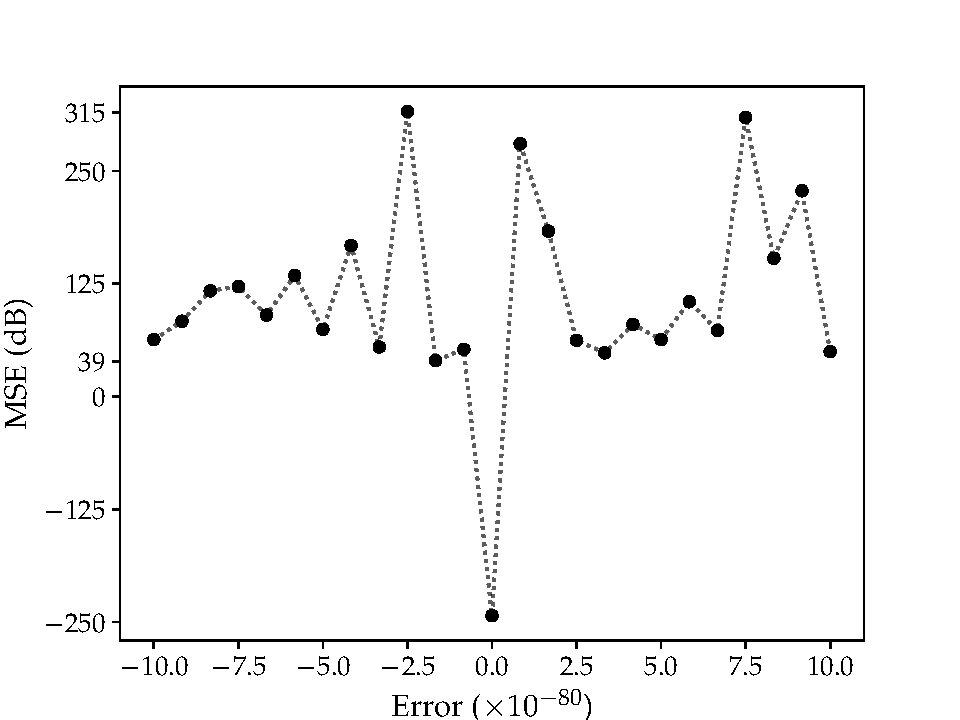
\includegraphics[width=10cm]{Figures/MSEdb_FrQDFT_EN.pdf}
\caption{Mean squared error, in dB, between the original and the decrypted images as function of the key error $ \epsilon $.}
\label{fig:MSE}
\end{figure}
%

Such an encryption scheme would not only be safe against brute-force attacks, given its key space dimension, but also known-plaintext attack. The reason for this is the non-linearity provided by the random-power block, as argued intensely by Hsue \parencite{hsue2018enhancing}. Resistance to chosen-plaintext attacks, however, is not guaranteed, although simple adjustments could be done in future works to address this problem: the vector of fractional orders $ \mathbf{a} = \{ a_0, a_1, \dots, a_{N-1} \} $ could be made dependent on both the plain image and external parameters (such as the secret seed $ s_0 $). Such tweak in the algorithm would block the extraction of information from comparing chosen plain images with their encrypted counterparts \parencite{chai2019color, hu2017chaotic, murugan2016image}, making the scheme resistant to chosen-plaintext and chosen-ciphertext attacks \parencite{wang2012novel}; with resistance also to the weaker attacks of brute-force and known-plaintext.

Alongside the investigation of key space dimension and sensitivity, histogram analysis play an important role in describing the performance of encryption schemes. A practical cipher should present an output symbol distribution ideally independent from the cleartext, so that no information is leaked through histogram visualization  \parencite{zhang2014symmetric}.
% "An ideal encrypted image should have a
% uniform and completely different histogram against the plain-image for preventing the adversary from extracting any mean-
% ingful information from the fluctuating histogram of the cipher-image." (zhang2014symmetric)
In the case of a PNG image, four histograms are drawn, one for each layer. Fig. \ref{fig:testing_hist} depicts a test PNG image split into its color and opacity components and the corresponding histograms, both prior and after encryption. A group of 13 $ 256\times 256 $-pixels PNG images were encrypted using the proposed method and the histograms of the ciphered output were collected, what is shown in Fig. \ref{fig:allhistograms}. No matter how diverse the input images may be, the histograms present continuously the same profile, what indicates decoupling of information between plain and ciphered images. Although a deeper study on the properties and safety standards of the proposed encryption scheme is needed for full description of its capacity, the analysis presented fit in the scope of this work and fulfill the goal of presenting the MFrQDFT with a clear and illustrative application.
%{\color{blue}Each image was ciphered using one of the following randomly defined keys (IMPLEMENTAR): $s_0 = $}. % For quantity analyses of each key, we employ variances of histograms to evaluate uniformity of ciphered images. The low-
% er value of variances indicates the higher uniformity of ciphered images. We also calculate the two variances of ciphered
% images which are encrypted by different secret keys on the same plaintext image. The closer of the two values of variances
% indicates the higher uniformity of ciphered images when the secret keys are varying. The variance of histograms is presented
% as follows:

%Histogram analysis: point out that the conversion from float to int, used prior to histogram-making, did not incur in information loss, because the MSE between the original image and the decrypted, AFTER CONVERSION, was
%MSE:  7.380345314385882e-25
%MSEint:  7.380345314385882e-25


\newcommand{\constlength}{0.5}

\begin{figure}[htbp]
\centering
\subfloat[]{
\includegraphics[width=0.35\linewidth]{Figures/alphatest_resized_decrypted.png}}~
\subfloat[]{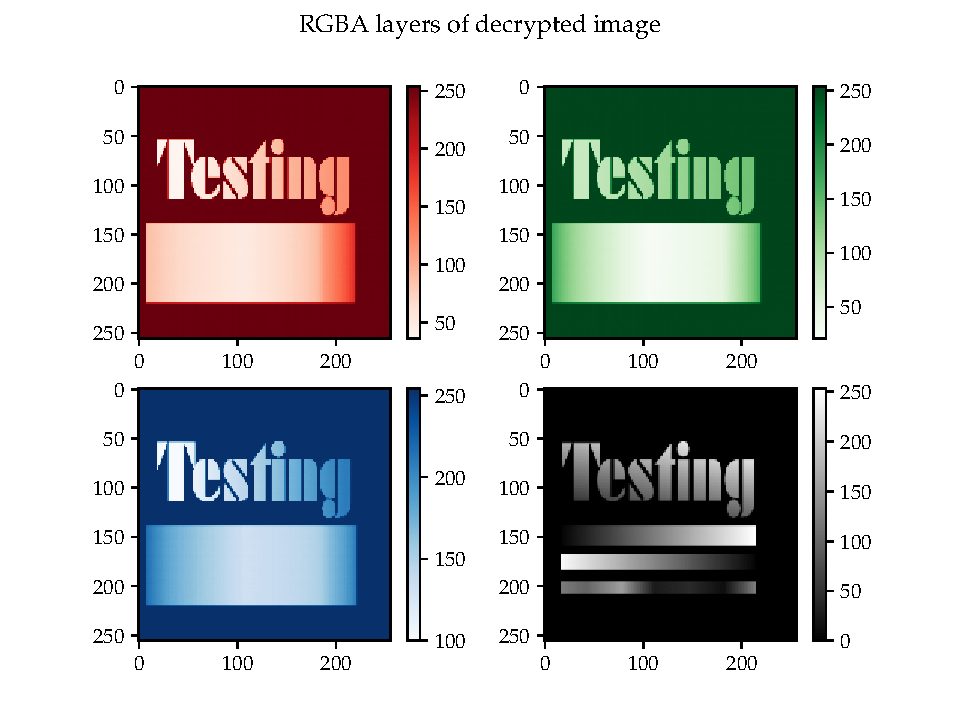
\includegraphics[width=\constlength\linewidth]{Figures/alphatest_resized_decrypted_RGBA_layers.pdf}} \\
\subfloat[]{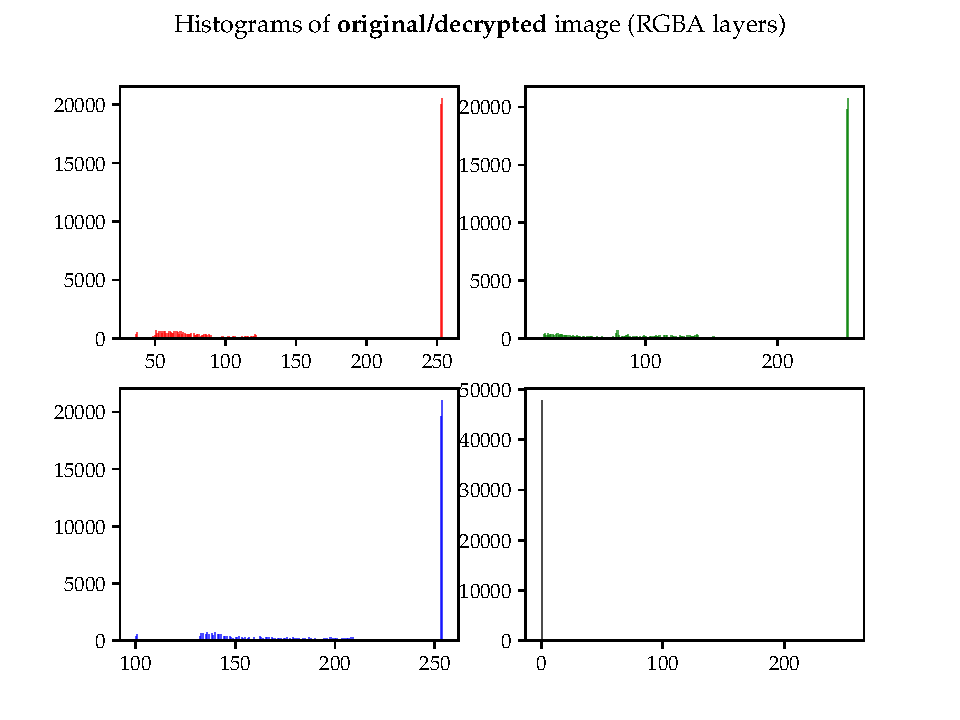
\includegraphics[width=\constlength\linewidth]{Figures/alphatest_resizeddecrypted_histograms.pdf}}~
\subfloat[]{
\includegraphics[width=0.3\linewidth]{Figures/alphatest_resized_encrypted_img.png}} \\
\subfloat[]{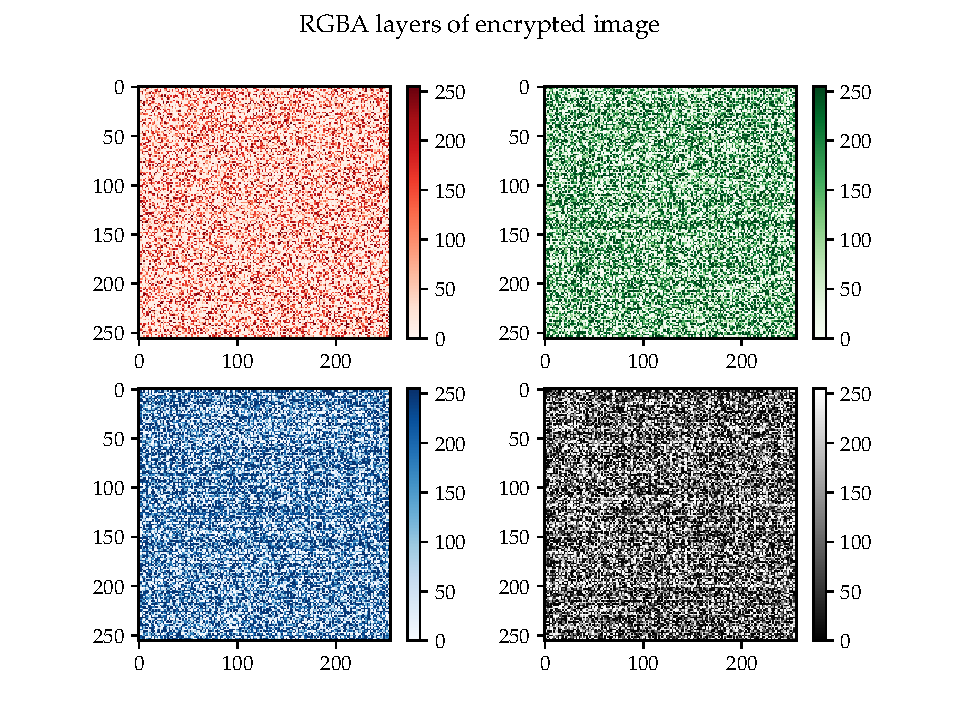
\includegraphics[width=\constlength\linewidth]{Figures/alphatest_resized_encrypted_RGBA_layers.pdf}}~
\subfloat[]{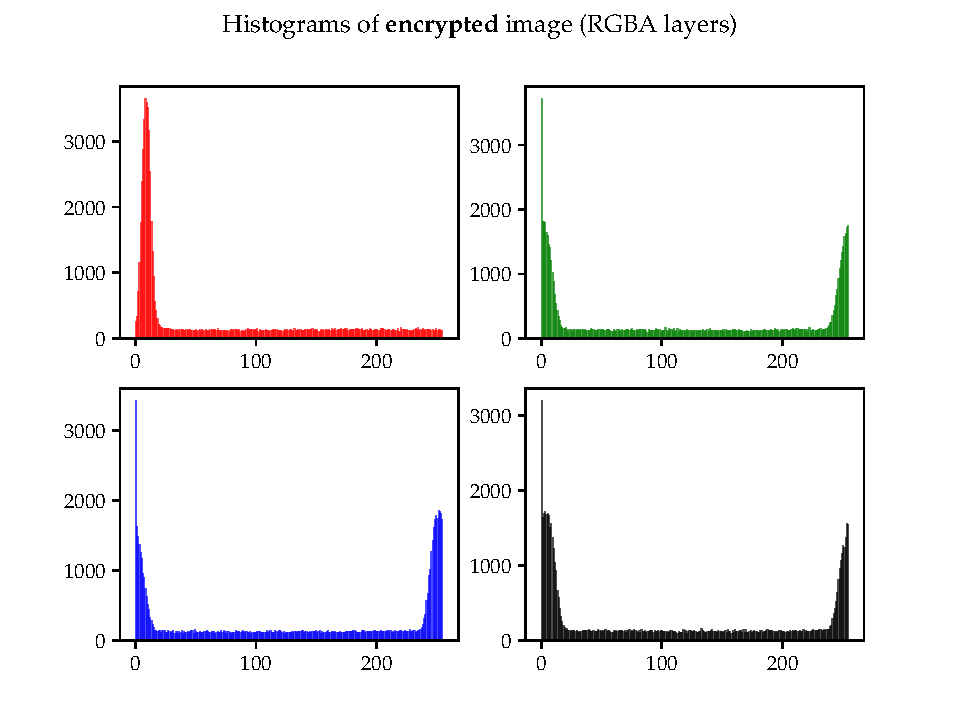
\includegraphics[width=\constlength\linewidth]{Figures/alphatest_resized_encrypted_histograms.pdf}}
\caption{(a) Test image in PNG format, with 256$ \times $256 pixels. (b) Color and opacity layers of the \textit{decrypted} image (which coincides with the original in (a)). (c) Histograms of each layer of the \textit{decrypted} image. (d) Encrypted image, in PNG format. (e) Color and opacity layers of the \textit{encrypted} image. (f) Histograms of each layer of the \textit{encrypted} image.}
\label{fig:testing_hist}
\end{figure}

\newcommand{\fixedlength}{0.35}
\newcommand{\smallerlength}{0.15}
\begin{figure}[htbp]
\centering
\subfloat[]{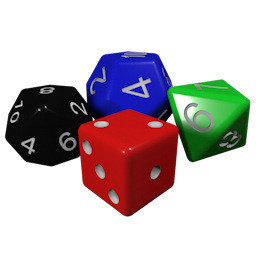
\includegraphics[width=\smallerlength\linewidth]{Figures/dice_256x256_decrypted.png}}~
\subfloat[]{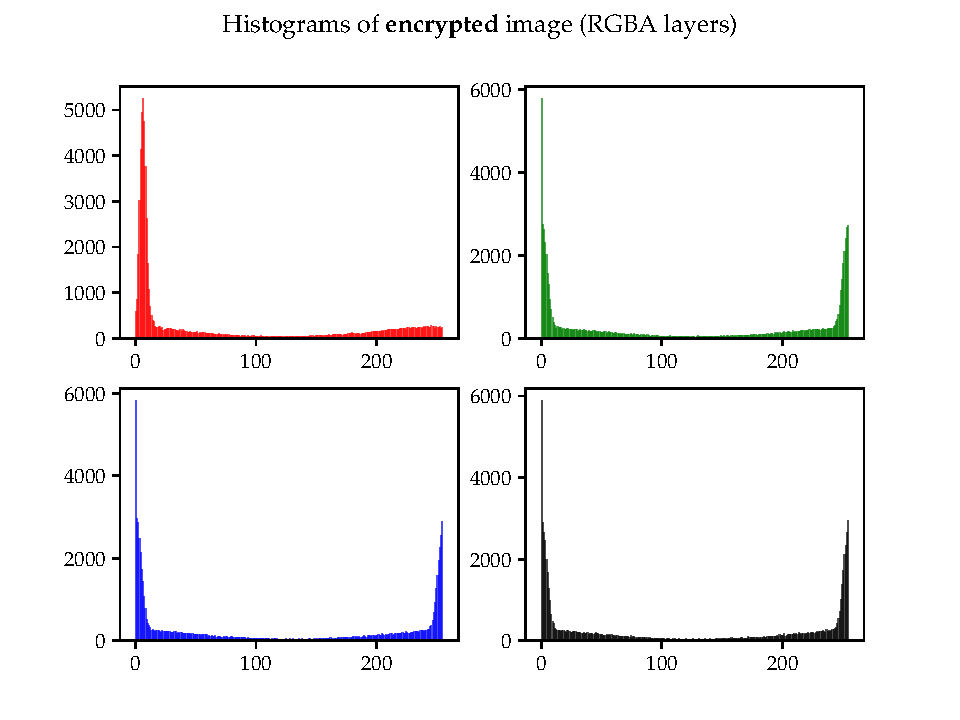
\includegraphics[width=\fixedlength\linewidth]{Figures/dice_256x256_encrypted_histograms.pdf}}~
\subfloat[]{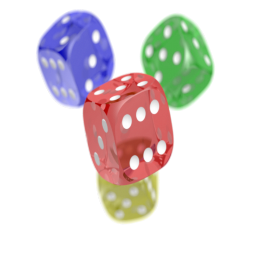
\includegraphics[width=\smallerlength\linewidth]{Figures/another_dice_resized_decrypted.png}}~
\subfloat[]{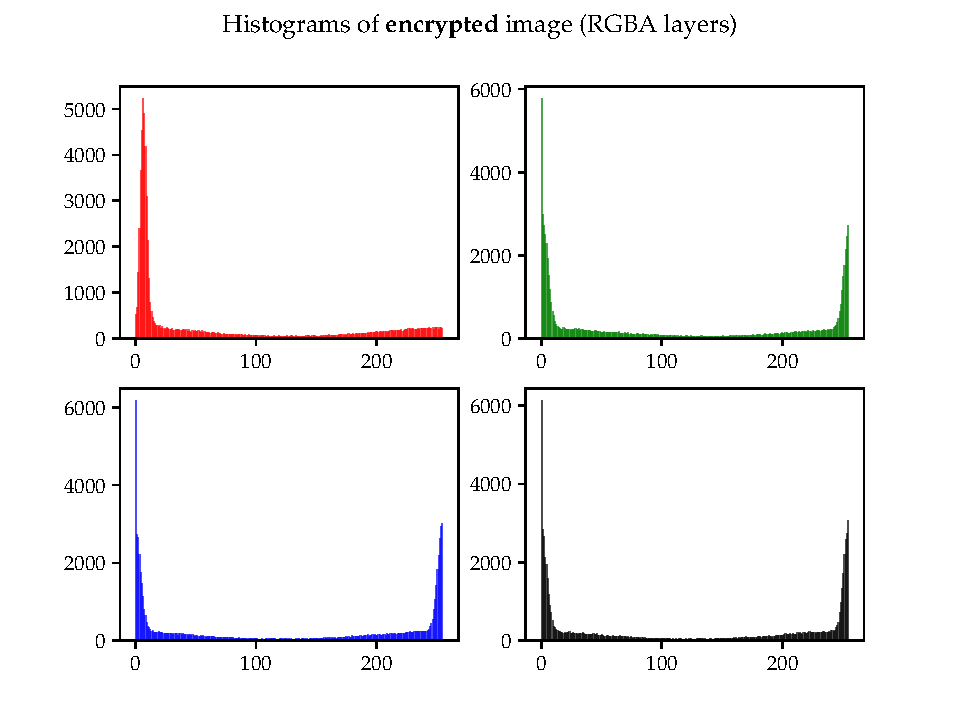
\includegraphics[width=\fixedlength\linewidth]{Figures/another_dice_resized_encrypted_histograms.pdf}}\\
\subfloat[]{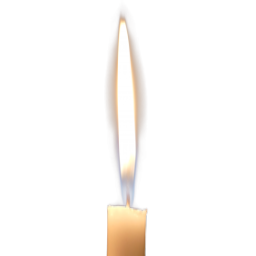
\includegraphics[width=\smallerlength\linewidth]{Figures/candle_resized.png}}~
\subfloat[]{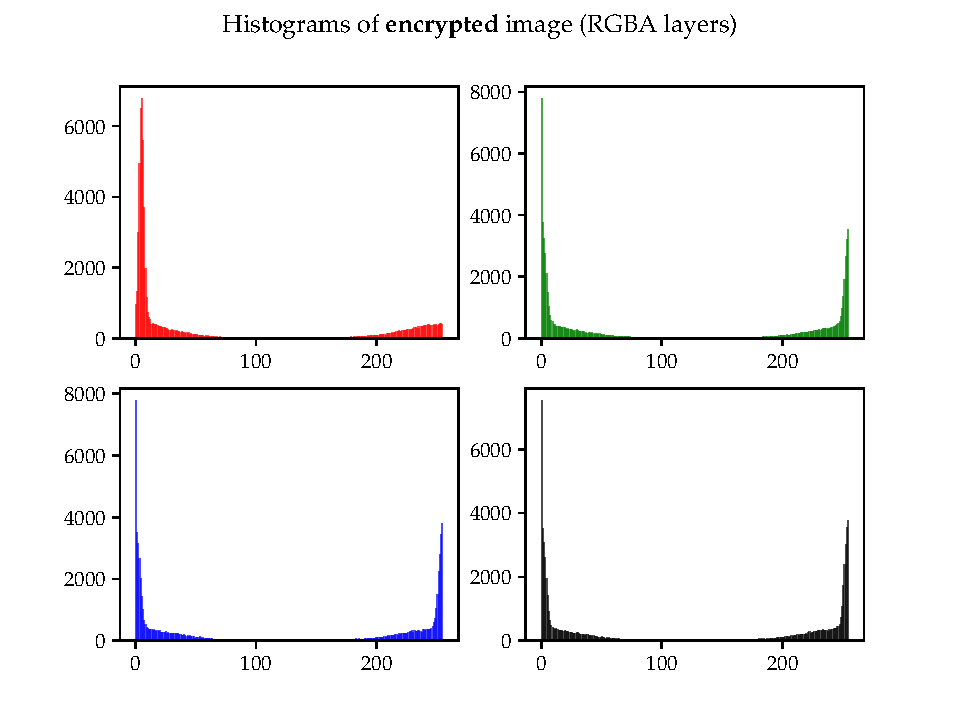
\includegraphics[width=\fixedlength\linewidth]{Figures/candle_encrypted_histograms.pdf}}~
\subfloat[]{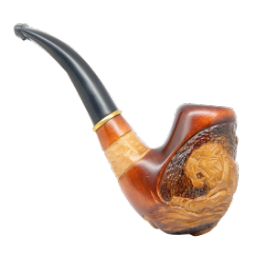
\includegraphics[width=\smallerlength\linewidth]{Figures/pipe_resized.png}}~
\subfloat[]{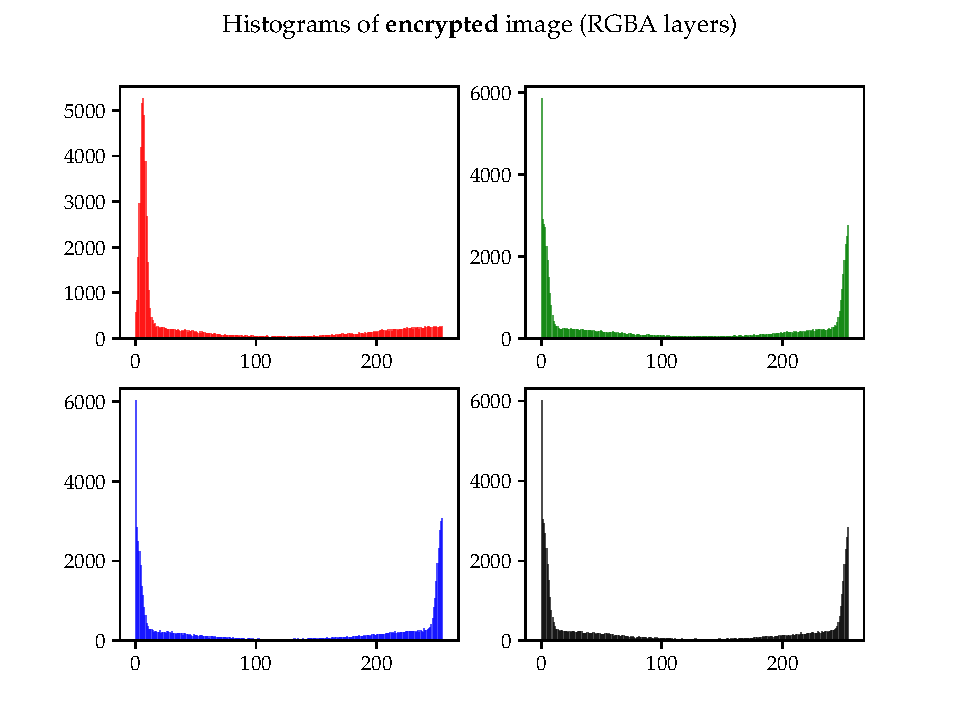
\includegraphics[width=\fixedlength\linewidth]{Figures/pipe_encrypted_histograms.pdf}}\\
\subfloat[]{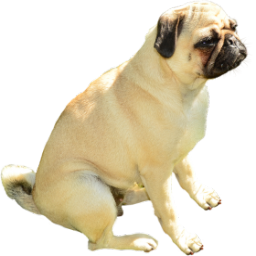
\includegraphics[width=\smallerlength\linewidth]{Figures/dog_resized.png}}~
\subfloat[]{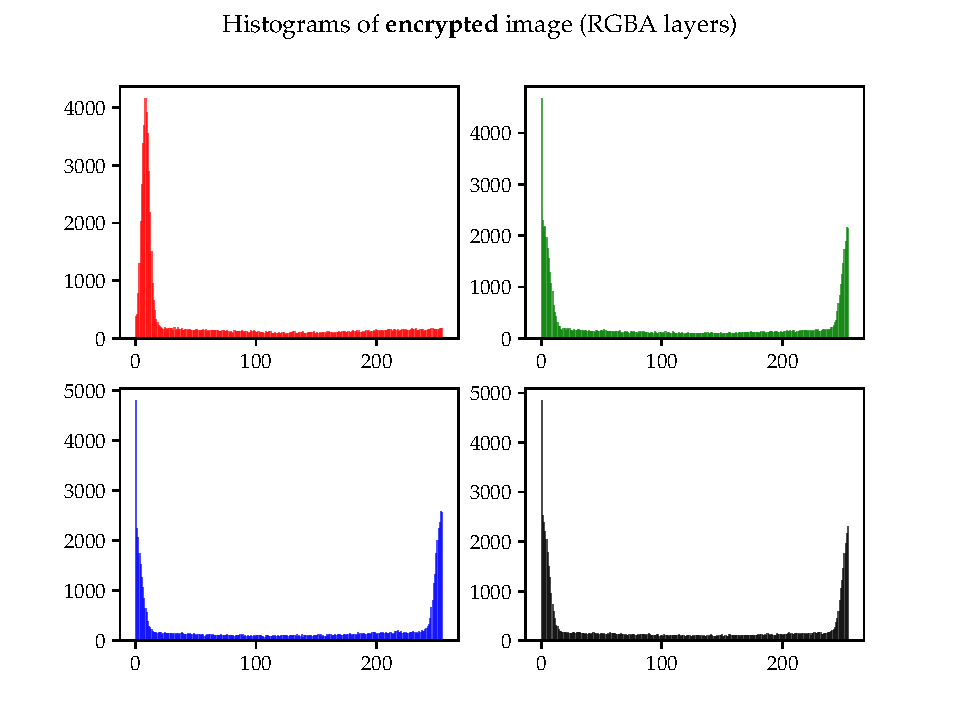
\includegraphics[width=\fixedlength\linewidth]{Figures/dog_encrypted_histograms.pdf}}~
\subfloat[]{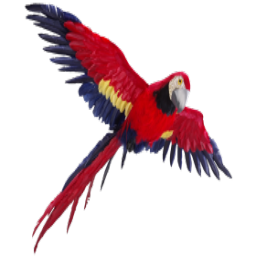
\includegraphics[width=\smallerlength\linewidth]{Figures/parrot_resized.png}}~
\subfloat[]{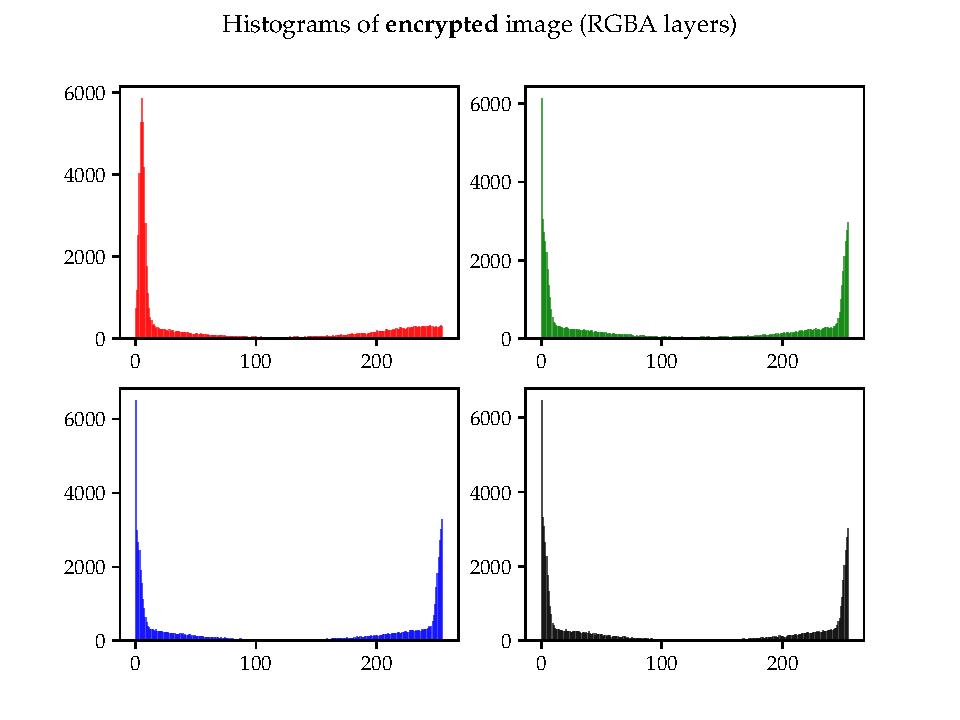
\includegraphics[width=\fixedlength\linewidth]{Figures/parrot_encrypted_histograms.pdf}}\\
\subfloat[]{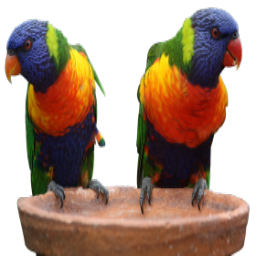
\includegraphics[width=\smallerlength\linewidth]{Figures/colorparrots_resized.png}}~
\subfloat[]{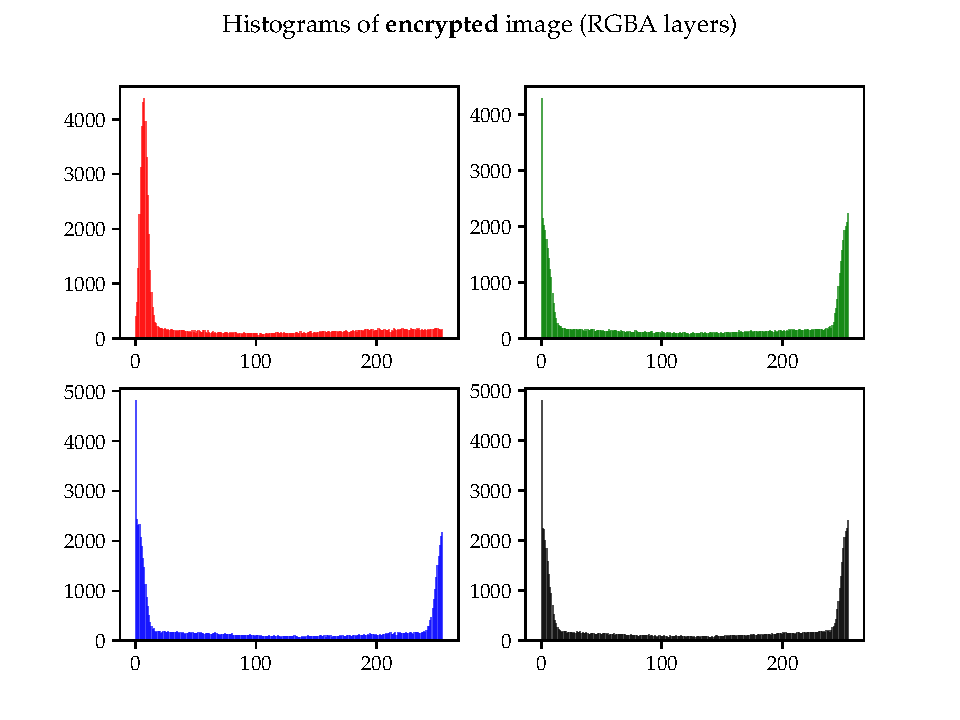
\includegraphics[width=\fixedlength\linewidth]{Figures/colorparrots_encrypted_histograms.pdf}}~
\subfloat[]{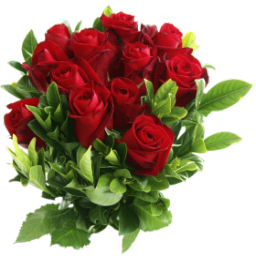
\includegraphics[width=\smallerlength\linewidth]{Figures/bouquet_resized.png}}~
\subfloat[]{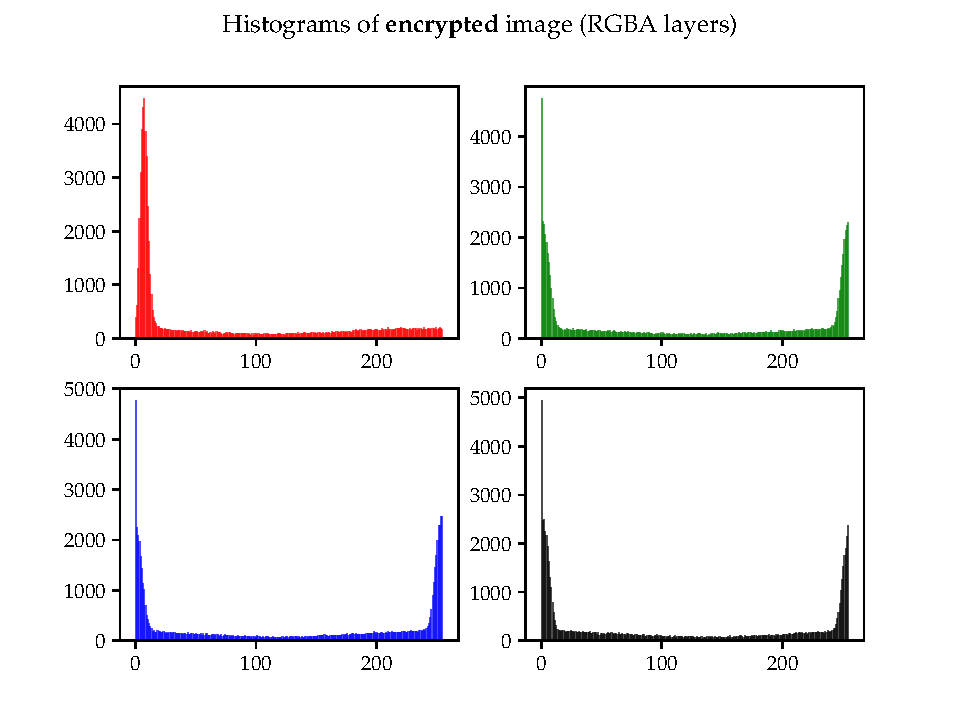
\includegraphics[width=\fixedlength\linewidth]{Figures/bouquet_encrypted_histograms.pdf}}

\vspace{3em}
\noindent \textit{(Part of Fig. \ref{fig:allhistograms}, it continues on the next page).}
%\caption{Legenda.}
\end{figure}

\stepcounter{figure}
\begin{figure}[htbp]
\centering
\ContinuedFloat
\subfloat[]{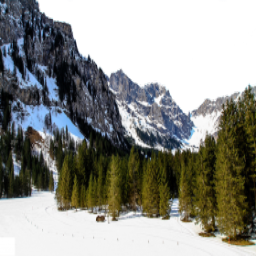
\includegraphics[width=\smallerlength\linewidth]{Figures/switzerland_resized.png}}~
\subfloat[]{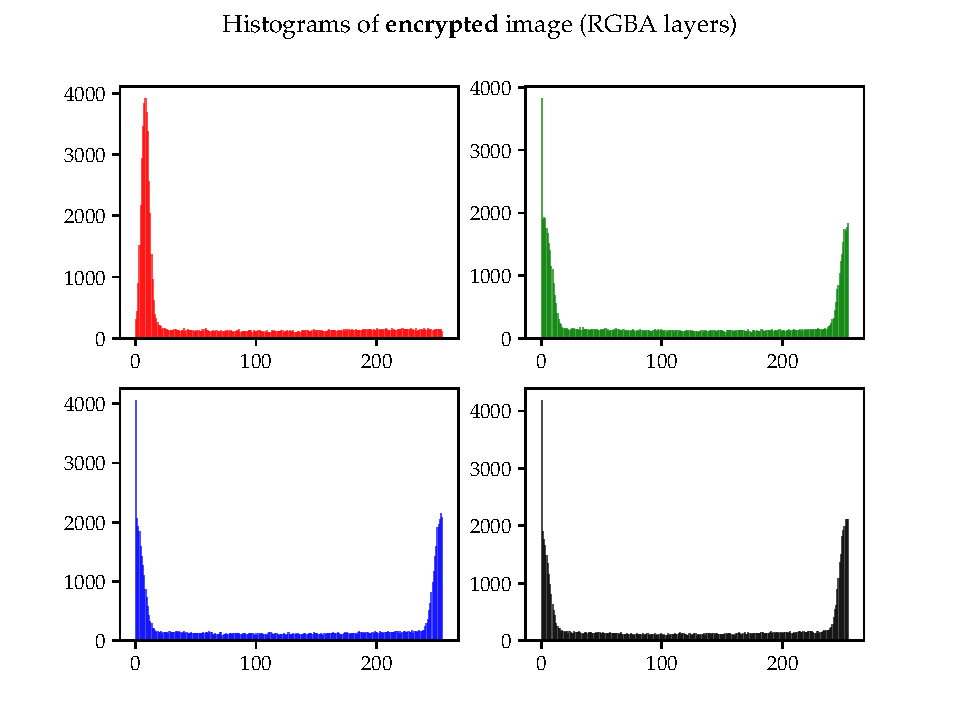
\includegraphics[width=\fixedlength\linewidth]{Figures/switzerland_encrypted_histograms.pdf}}~
\subfloat[]{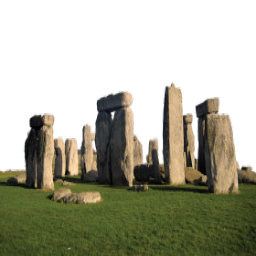
\includegraphics[width=\smallerlength\linewidth]{Figures/london_resized.png}}~
\subfloat[]{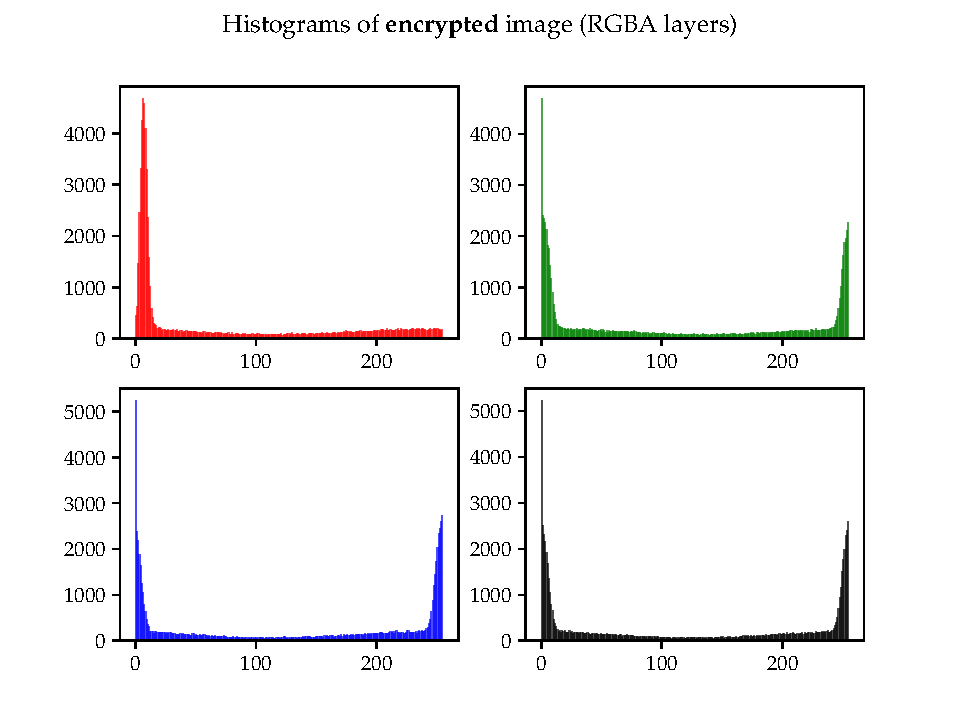
\includegraphics[width=\fixedlength\linewidth]{Figures/london_encrypted_histograms.pdf}}\\
\subfloat[]{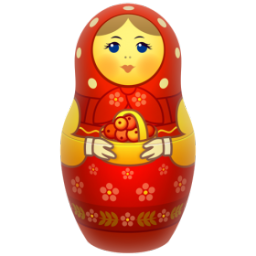
\includegraphics[width=\smallerlength\linewidth]{Figures/russia_resized.png}}~
\subfloat[]{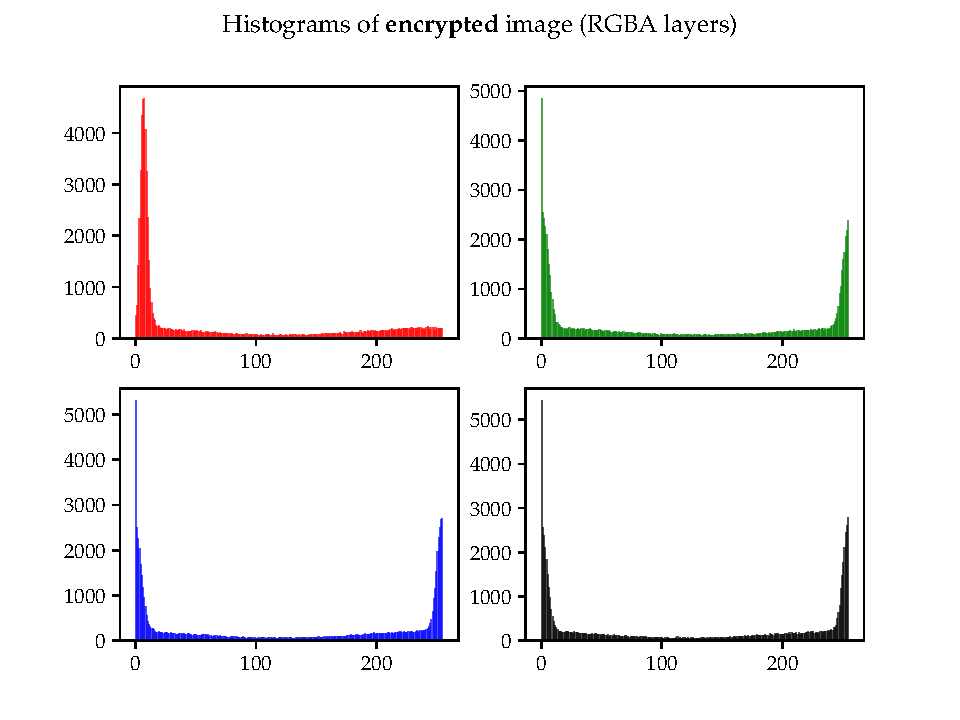
\includegraphics[width=\fixedlength\linewidth]{Figures/russia_encrypted_histograms.pdf}}~
\subfloat[]{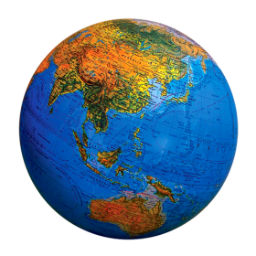
\includegraphics[width=\smallerlength\linewidth]{Figures/globe_resized.png}}~
\subfloat[]{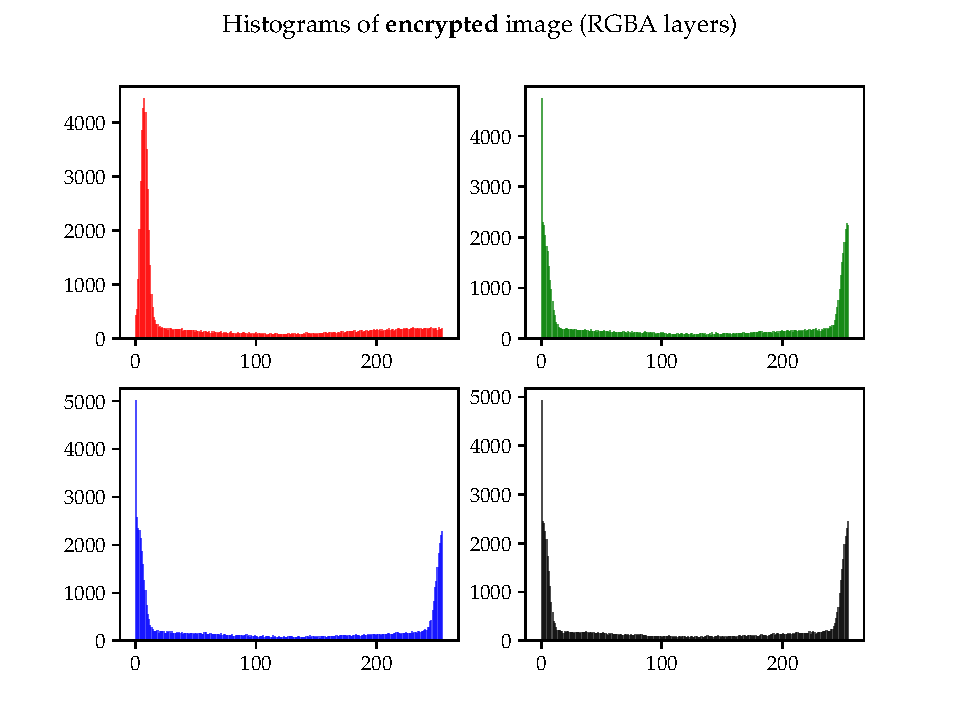
\includegraphics[width=\fixedlength\linewidth]{Figures/globe_encrypted_histograms.pdf}}\\
\subfloat[]{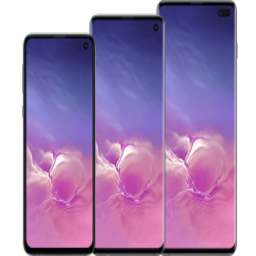
\includegraphics[width=\smallerlength\linewidth]{Figures/phones_resized.png}}~
\subfloat[]{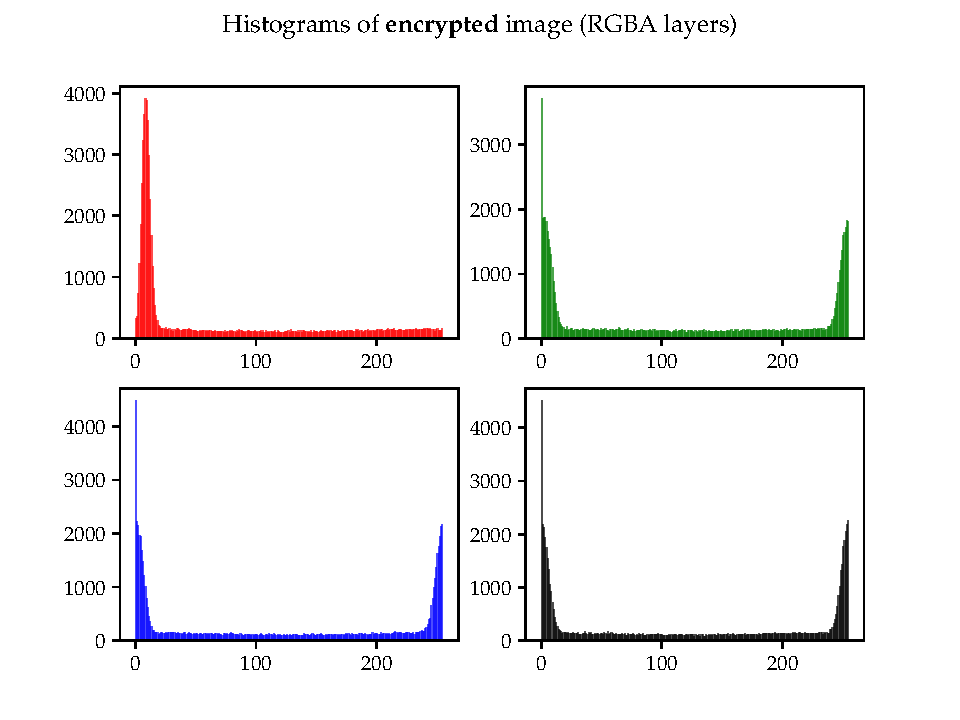
\includegraphics[width=\fixedlength\linewidth]{Figures/phones_encrypted_histograms.pdf}}
\caption{Set of 13 PNG test images, 256$ \times $256 pixels, alongside the histograms of each layer (colors and opacity) of their encrypted version. Images downloaded from the online free database \texttt{https://purepng.com/}, under CC0 license.}
\label{fig:allhistograms}
\end{figure}

Finally, as stated at the beginning of the chapter, there are a multitude of studies on image encryption, each addressing particular aspects and problems. Therefore, it is adequate to acknowledge the position of this proposed encryption algorithm in the literature landscape. Without providing an extensive and complete analysis, for lack of space, some remarks can be done. The key space dimension in related works vary from circa $ 10^{54} $, around 160 bits, in a work by Wang \textit{et al.} with flexible key space \parencite{wang2015novel}, to more than 400 bits, in a paper by Zhang \textit{et al.} \parencite{zhang2015new}, an interval which includes the 260 bits of the proposed algorithm. Regarding time of encryption, Wang \textit{et al.} \parencite{wang2015novelchaotic} used Arnold cat map and dynamic random growth to obtain large running speed of the encryption and decryption algorithm. This is an aspect our proposed scheme is not optimized for, although great improvement in processing time can be achieved if the eigenvector and eigenvalue matrices of the QDFT are stored in-memory, taking the eigendecomposition out of the encryption process. As a final comment, the main advantages of the proposed scheme are its modularization, the holistic processing of color images with opacity layer, the lack of long iterations and the ease to describe, comprehend and implement.

\section{Concluding remarks}
\label{sec:conclusao}
This chapter investigated the eigenstructure of the quaternion discrete Fourier transform. Although quaternion matrix decomposition is a challenging topic, the problem for the QDFT was solved by proving that this transform and the DFT share symmetric eigenvectors, what allowed for the construction of an orthogonal eigenbasis of the QDFT, using Hermite--Gaussian-like DFT eigenvectors \parencite{de2017discrete}. This result led to the definition of a fractional QDFT, which was proven to hold properties similar to those of the FrDFT, its complex-valued counterpart.

The FrQDFT was further generalized by introducing the MFrQDFT, a multiparametric version. Exploring the 4D nature of quaternions, a holistic encryption scheme for color images with opacity layer was proposed, as an illustrative application of the 2D-MFrQDFT, and shown to provide satisfactorily large key space and key sensitivity, resistance to known-plaintext attack and ease of description and implementation. Future works could possibly expand this analysis and address whether some hypercomplex image moments, such as ternary radial harmonic Fourier moments and quaternion polar harmonic \parencite{wang2019ternary,wang2018quaternion}, could be used for image encryption, eventually in specific scenarios and applications.
